%%%%%%%%%%%% Selective edge pruning %%%%%%%%%%%%
\chapter{Selective edge pruning uncovers subset of regulatory genes} \label{s:ap:sel_prun}

% Leiden vs SBM
\section{Leiden vs SBM} \label{s:ap:leiden_sbm}

The below figures are supporting the work presented in \cref{s:N_I:sel_tf_com_det} where the two set of traces, one for Leiden (\cref{fig:ap:sbm_com_size}) and one for SBM (\cref{fig:ap:sbm_com_size}), are shown in a single figure in \cref{fig:N_I:comp_size_com_det}. 

The advantage of showing the two figures separately is that the variance in the community size is illustrated clearly as well as the difference in the number of communities found.

% Comunity sizes
\begin{figure}[!h]
    \centering
    \begin{subfigure}[!t]{1.0\textwidth}
        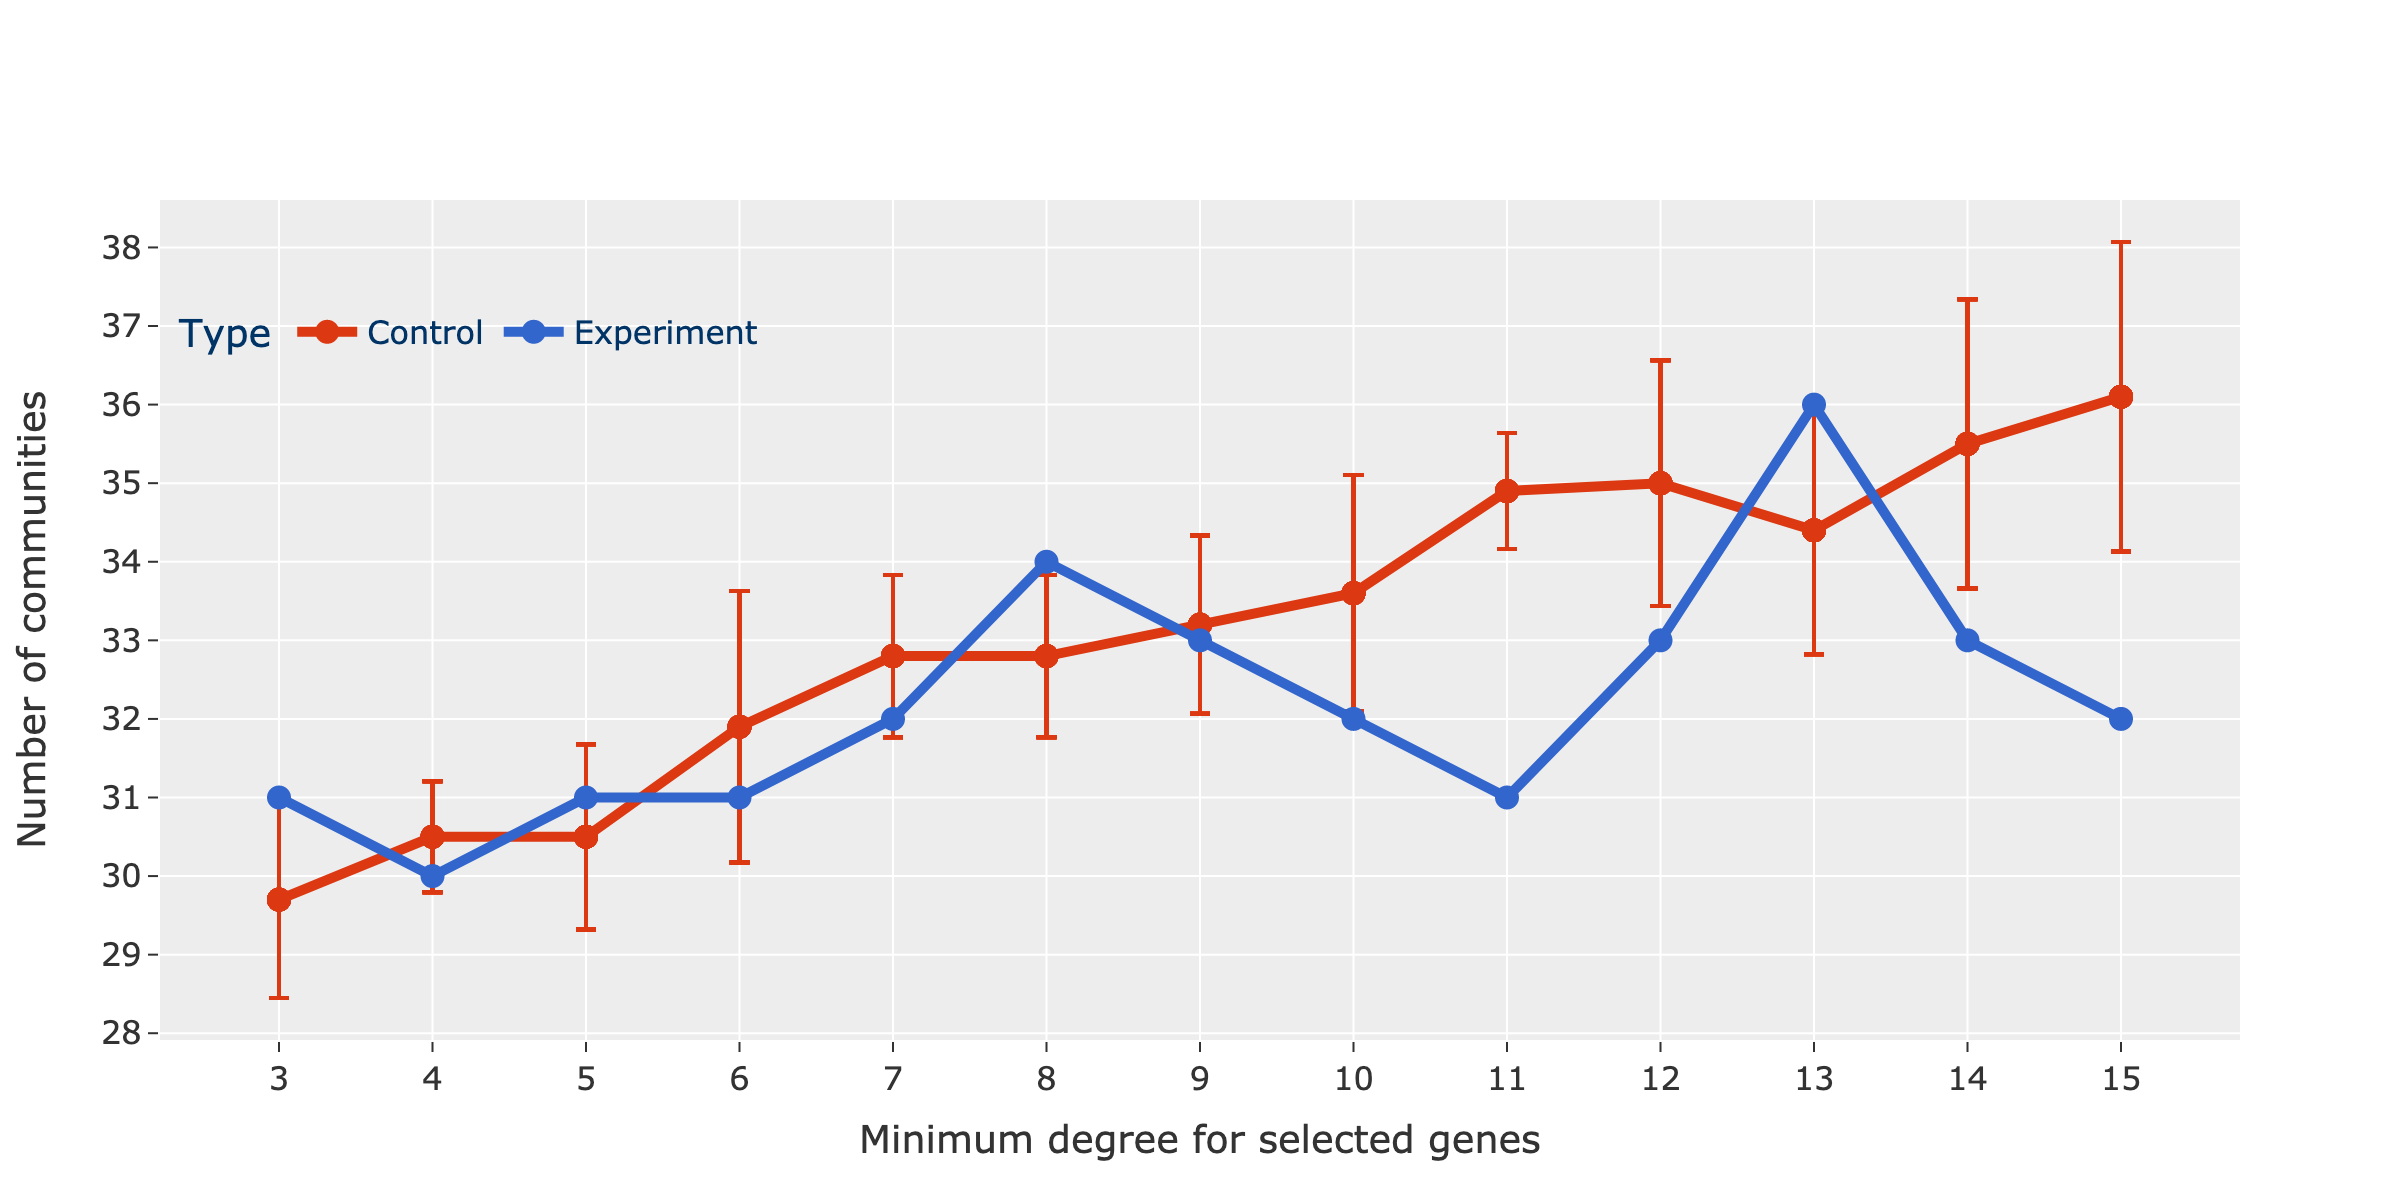
\includegraphics[width=\textwidth]{Sections/Network_I/Resources/selective_pruning/com_comp/sbm_comNum_sel_prun.png}
        \caption{SBM}
        \label{fig:ap:sbm_com_size}
    \end{subfigure} 
    \begin{subfigure}[!t]{1.0\textwidth}
        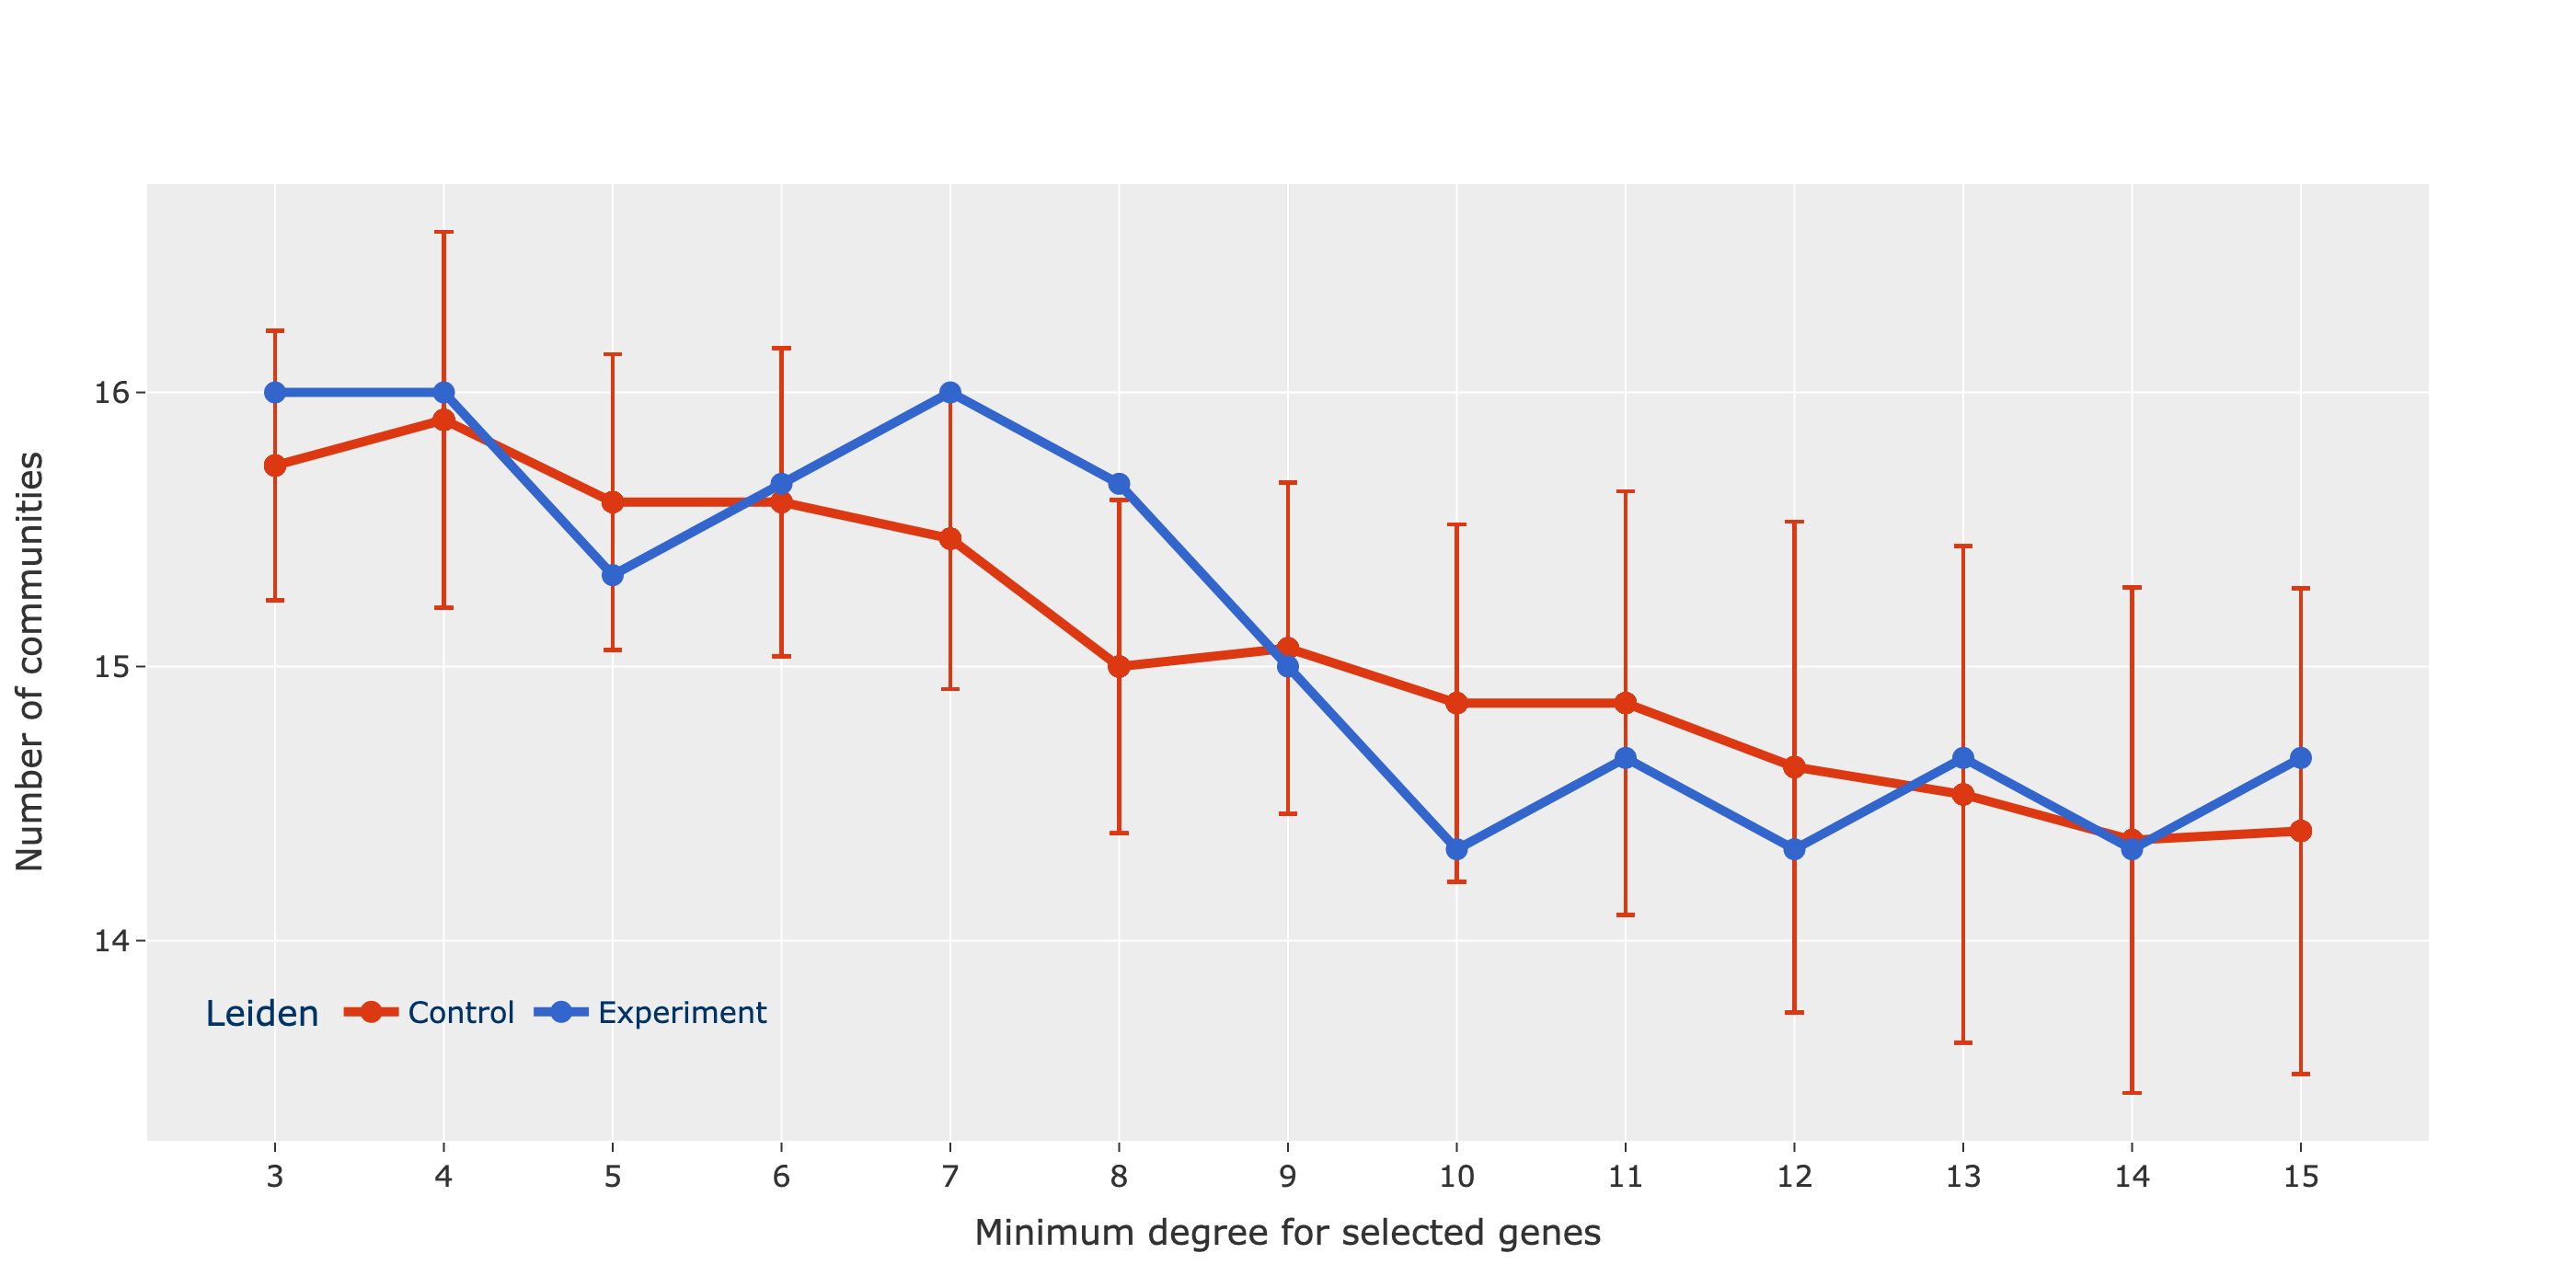
\includegraphics[width=\linewidth]{Sections/Network_I/Resources/selective_pruning/leid_comNum_sel_prun.png}
        \caption{Leiden}
        \label{fig:ap:leid_com_size}
    \end{subfigure}\hspace{\fill}  
    \caption[Leiden vs SBM: community size comparison]{Community size comparison between Leiden and SBM. This serves as a supporting material to the work done in \cref{s:N_I:sel_pruning}. It shows that SBM tends to find more communities compared to Leiden.}
    \label{fig:ap:com_size_comp}
\end{figure}

% Cluster analysis
\section{Cluster analysis} \label{s:ap:sel_tfs_cs}

The clustering analysis below supports the MIBC groups found using the expression of the 98 TF genes which are highly correlated with other genes in the tumour network, see \cref{s:N_I:sel_tfs_mibc}.

% Talk about the clustering
Hierarchical clustering was applied to the tumour expression of the 98 TF after 11 samples previously identified as outliers were removed\footnote{In this context, outliers are samples that cluster in 1-3 groups, making it hard to interpret the dendrogram from the hierarchical clustering}, leaving 392 samples for clustering. The tumour\footnote{TCGA's MIBC cohort} data was log2(TPM+1) transformed, normalised by the quantiles, and then agglomerative clustering with average linkage was applied on the 1-Pearson correlation distance\footnote{In this case, for both clustering and visualisation, Morpheus from the Broad Institute was used \cite{Broad-Institute2016-tn}}. This method was preferred over those developed in the previous chapter because the number of genes was small and the heatmap from Morpheus is a useful tool for showing the gene expression specific to a group. The heatmap and the output are shown in \cref{fig:ap:morph_sel_tfs} in the Appendix.

% describe morpheus
A dendrogram cut of 15 was chosen as it split both the Luminal and Basal Groups and there are relatively small groups. From the heatmap \cref{fig:ap:morph_sel_tfs} it can be noticed that there is a large group of Luminal samples and a smaller one. The Basal group is split into three subgroups, a large one, a medium size which groups most of the Mes-like tumours from Lund classifier and a smaller ones which has a lower Infiltration/Stromal/Estimate scores compared to the other 2 Basal groups. Apart from these 2 groups, there are outliers samples that are grouped in 1 or 2 clusters, suggesting that they have particular molecular profiles.

The groups smaller than 1\% of the cohort size (equivalent to 4 samples) are removed, resulting in a dataset of 378 samples grouped into 5 major groups. 


%  Morpheus hierarchical clustering
% \begin{figure}[!htb]   
\begin{sidewaysfigure}
    \centering
    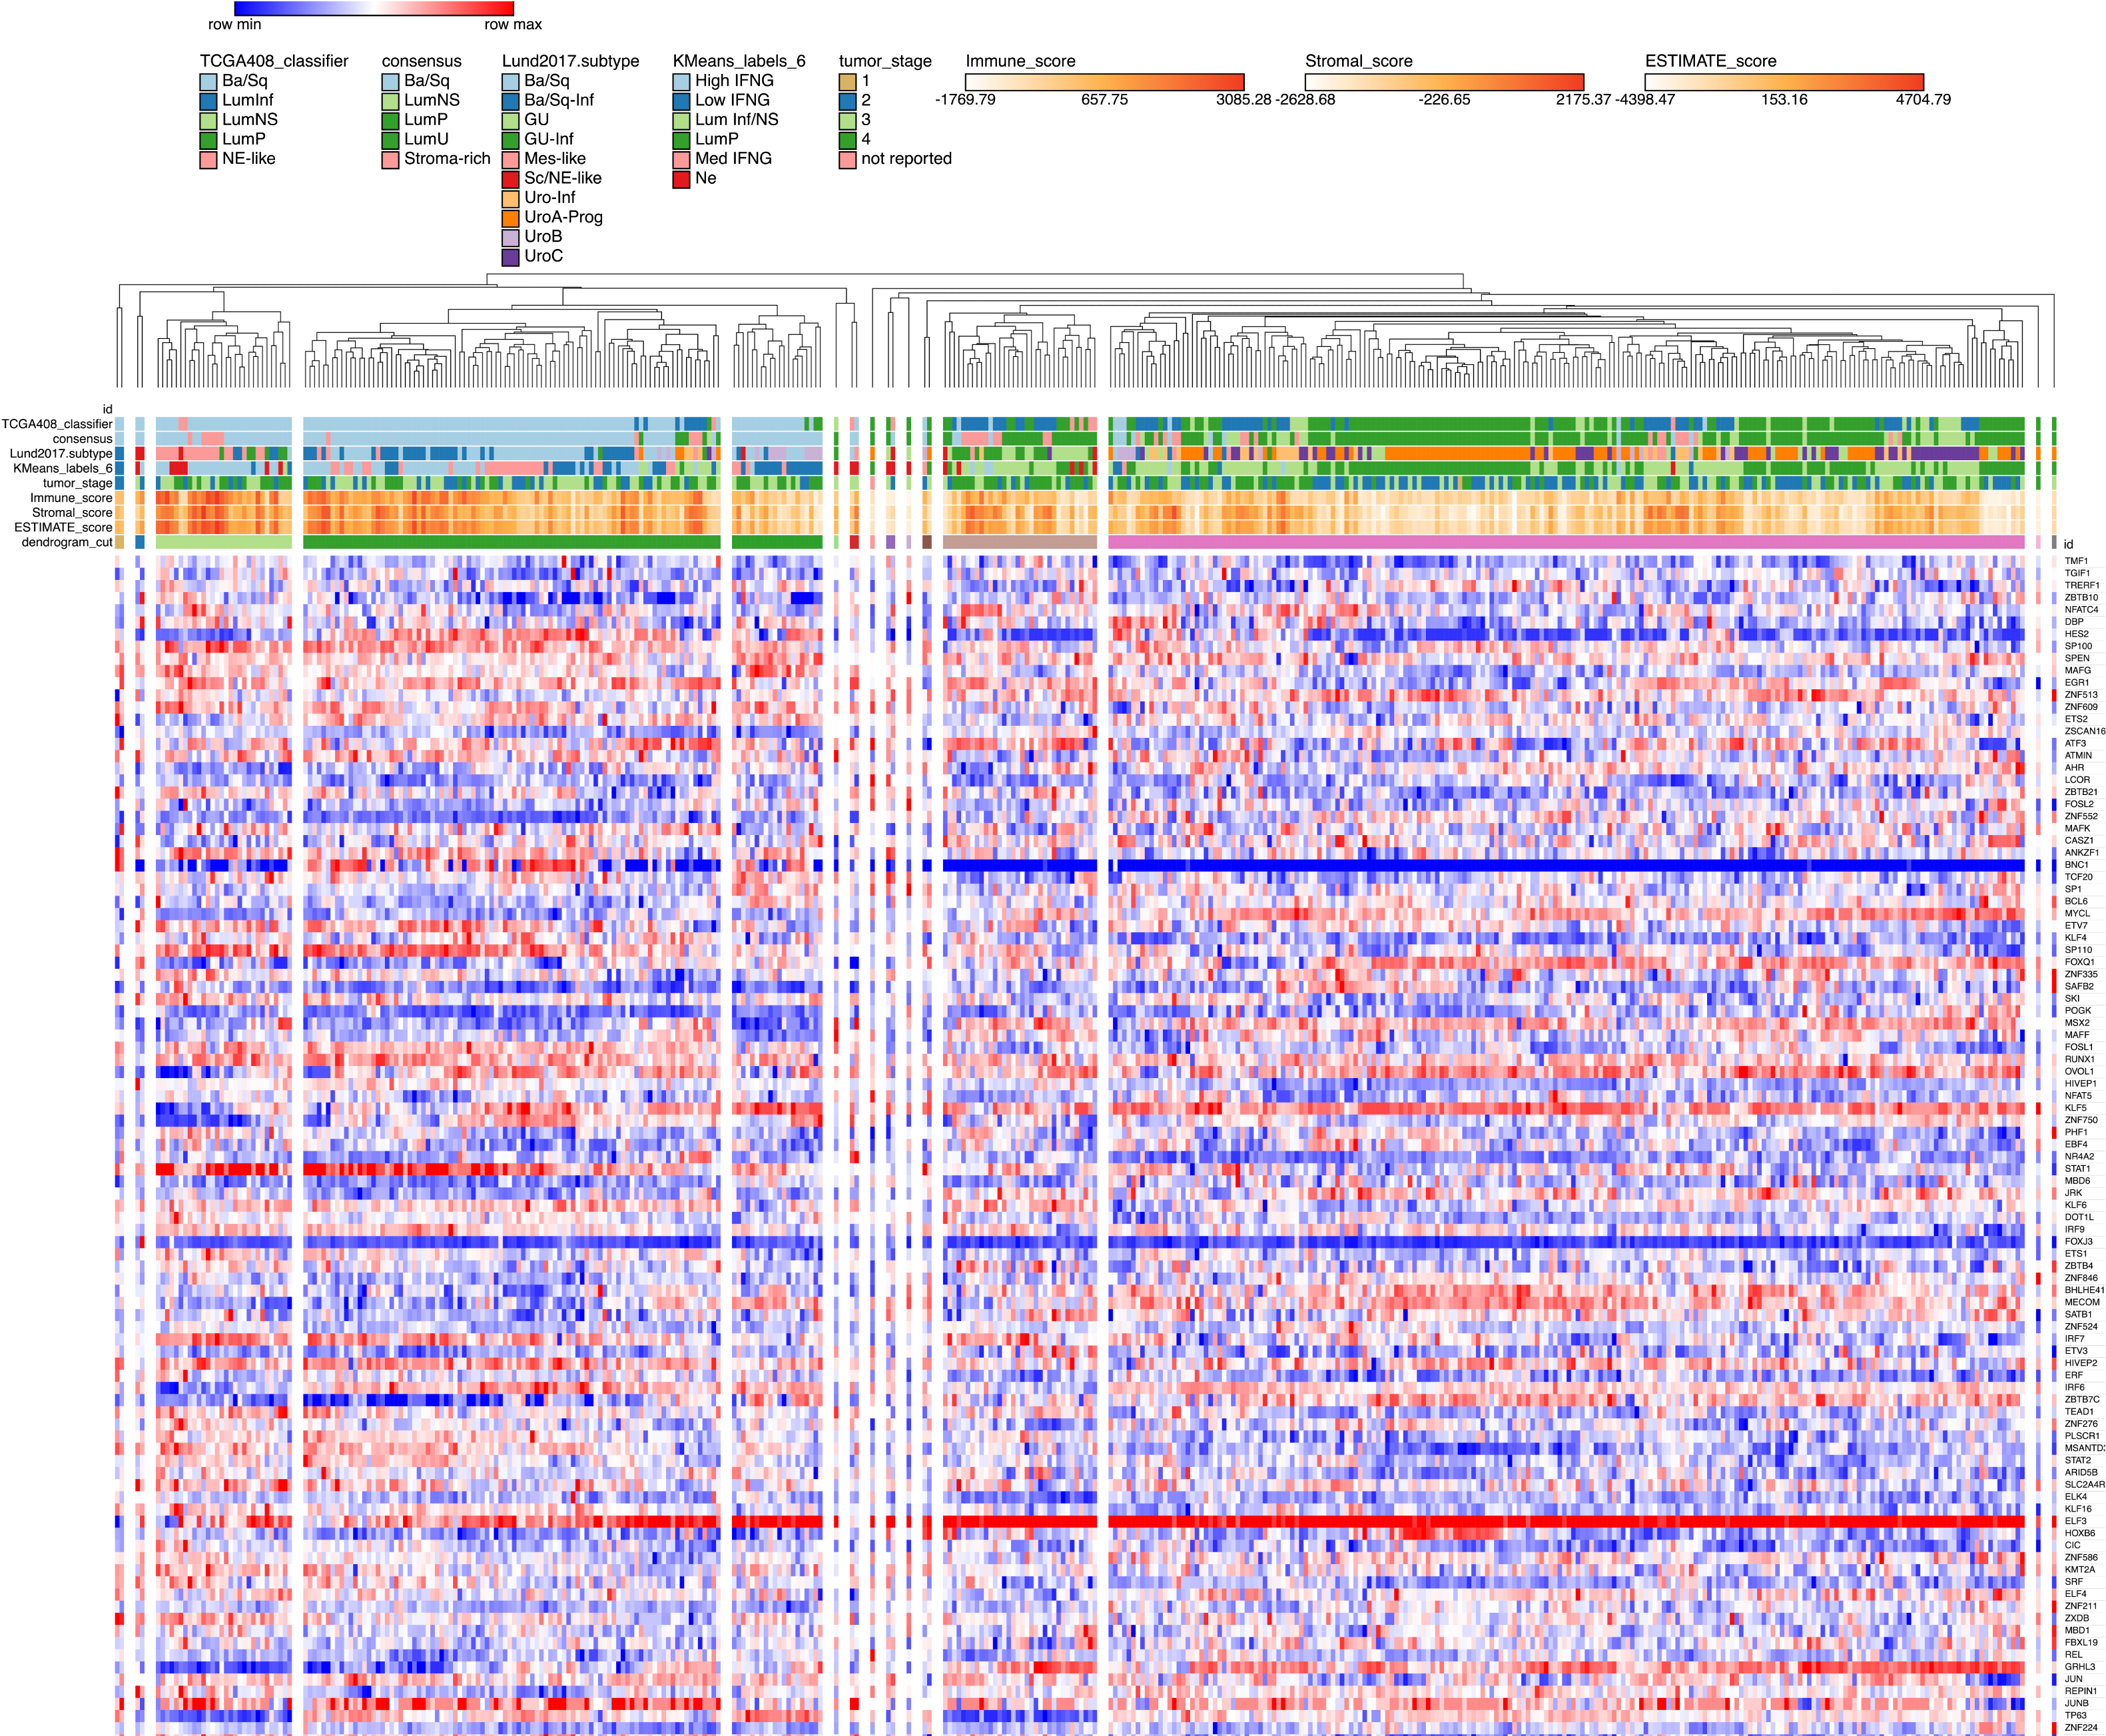
\includegraphics[width=1.0\textwidth,keepaspectratio]{Sections/Network_I/Resources/selective_pruning/15_CS_norm_sel_tfs.png}
      \caption[Heatmap of the clustering of the gene expression of the 98 TF]{Hierarchical clustering of the 98 TF found in \cref{s:N_I:sel_tfs}. 
      Their gene expression was log2(TPM+1) transformed, normalised by the quantiles, and then agglomerative clustering with average linkage was applied on the 1-Pearson correlation distance. The columns at the top of the heatmap represents the previous classification (TCGA \cite{Robertson2017-mg}, Consensus \cite{Kamoun2020-tj}, Lund \cite{Marzouka2018-ge} and the stratification from \cref{s:clustering_analysis}) as well as the Immune, Stromal and ESTIMATE scores available with the TCGA cohort.}
    \label{fig:ap:morph_sel_tfs}
\end{sidewaysfigure}

% tumour vs non-tumour
\section{Tumour vs Non-tumour gene expression} \label{s:ap:tum_vs_non-tumour}


The scatter plot complements the work in \cref{s:N_I:sel_tfs_bio} which explores the 98 TF in both tumour and non-tumour datasets.

\Cref{fig:ap:sel_tfs_mean} depicts the mean expression of the 98 TF genes found in the previous subsection. The log plot shows the non-cancerous mean on the y-axis and the tumour mean expression on the x-axis, the size and colour of the points is proportional to the mutation burden across the MIBC cohort from TCGA. The genes higher on the y-axis have a higher expression in the non-cancerous, similarly for x-axis, further on the right hand side, higher average value in the tumour cohort. \textit{ELF3} it is on the top right corner meaning that it is expressed both in the tumour and non-cancerous datasets, and it is also highly mutated in MIBC. \textit{BNC1} is on he left corner, having lower expression across the samples.

% Tum vs non-cancerous dataset.
\begin{figure}[!htb]
    \centering
    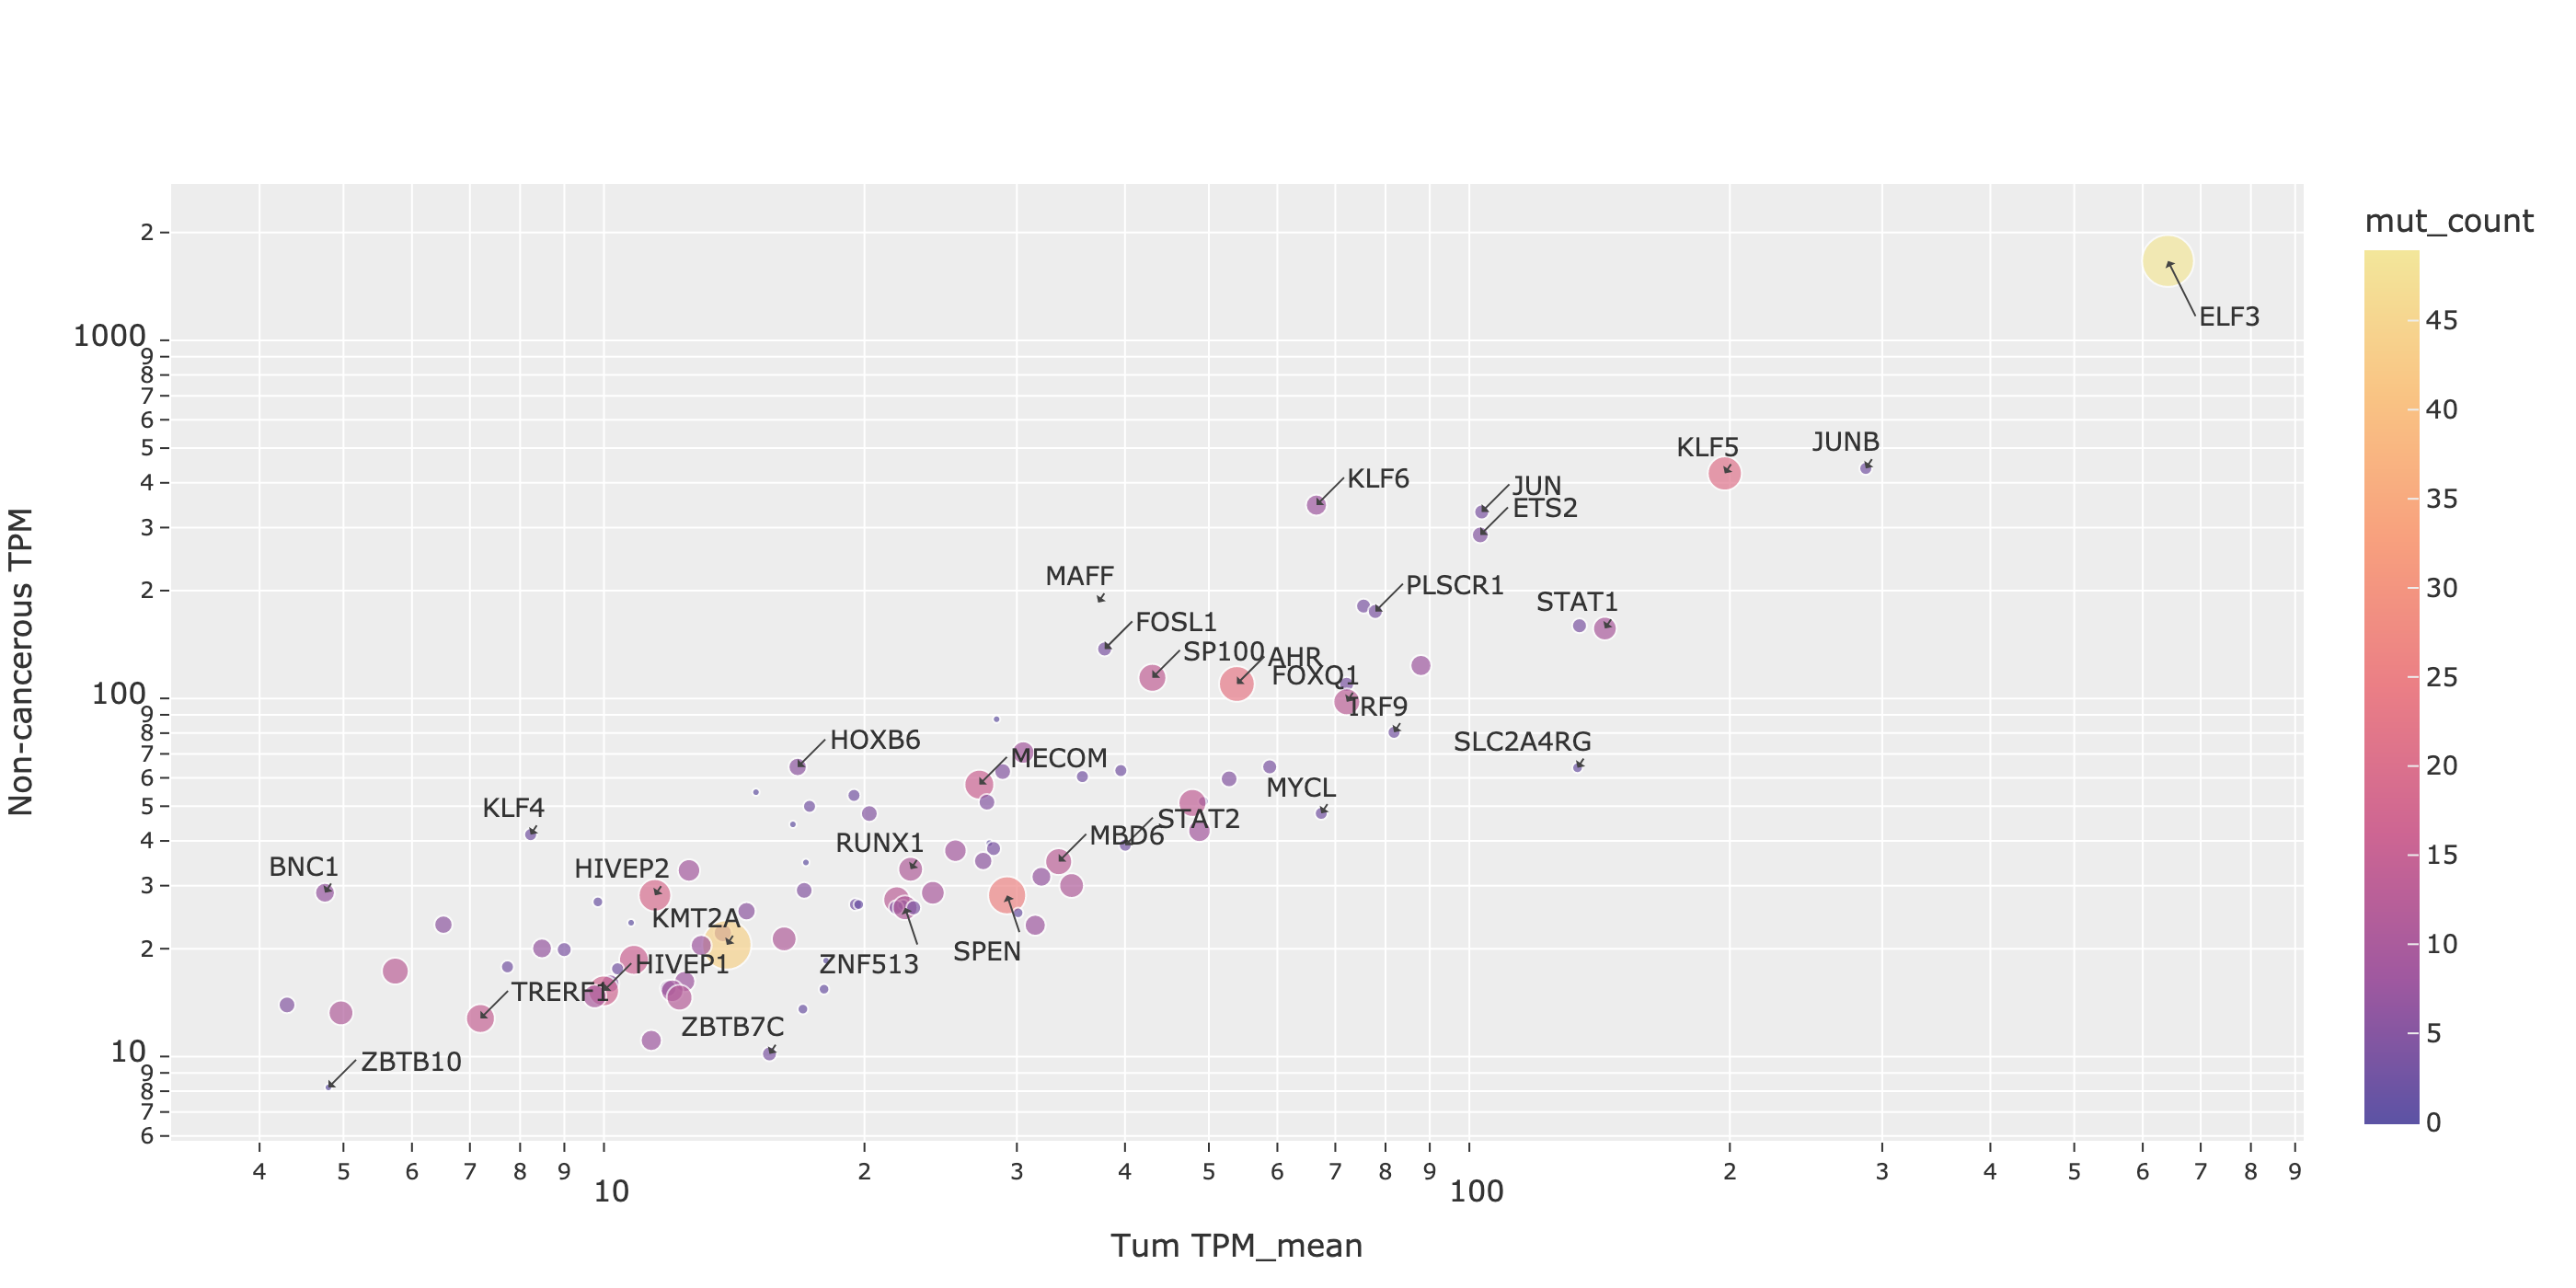
\includegraphics[width=1.0\textwidth,keepaspectratio]{Sections/Network_I/Resources/selective_pruning/sel_tfs/sel_tfs_mean_tum_healthy.png}
    \caption[Tumour vs non-tumour gene expression of the 98 TF]{Selected TF expression in the MIBC TCGA cohort and in the non-cancerous. Both the colour and size of the points are proportional to the mutation burden in the TCGA cohort.}
    \label{fig:ap:sel_tfs_mean}
\end{figure}


% Basal/consensus subgroups
\section{Basal and Luminal markers on consensus subgroups} \label{s:ap:sel_prun_markers}

% The Basal/Luminal Markers in the consensus
\begin{figure}[!htb]
    \captionsetup[subfigure]{justification=Centering}
  % consensus
  \begin{subfigure}[!t]{0.95\textwidth}
    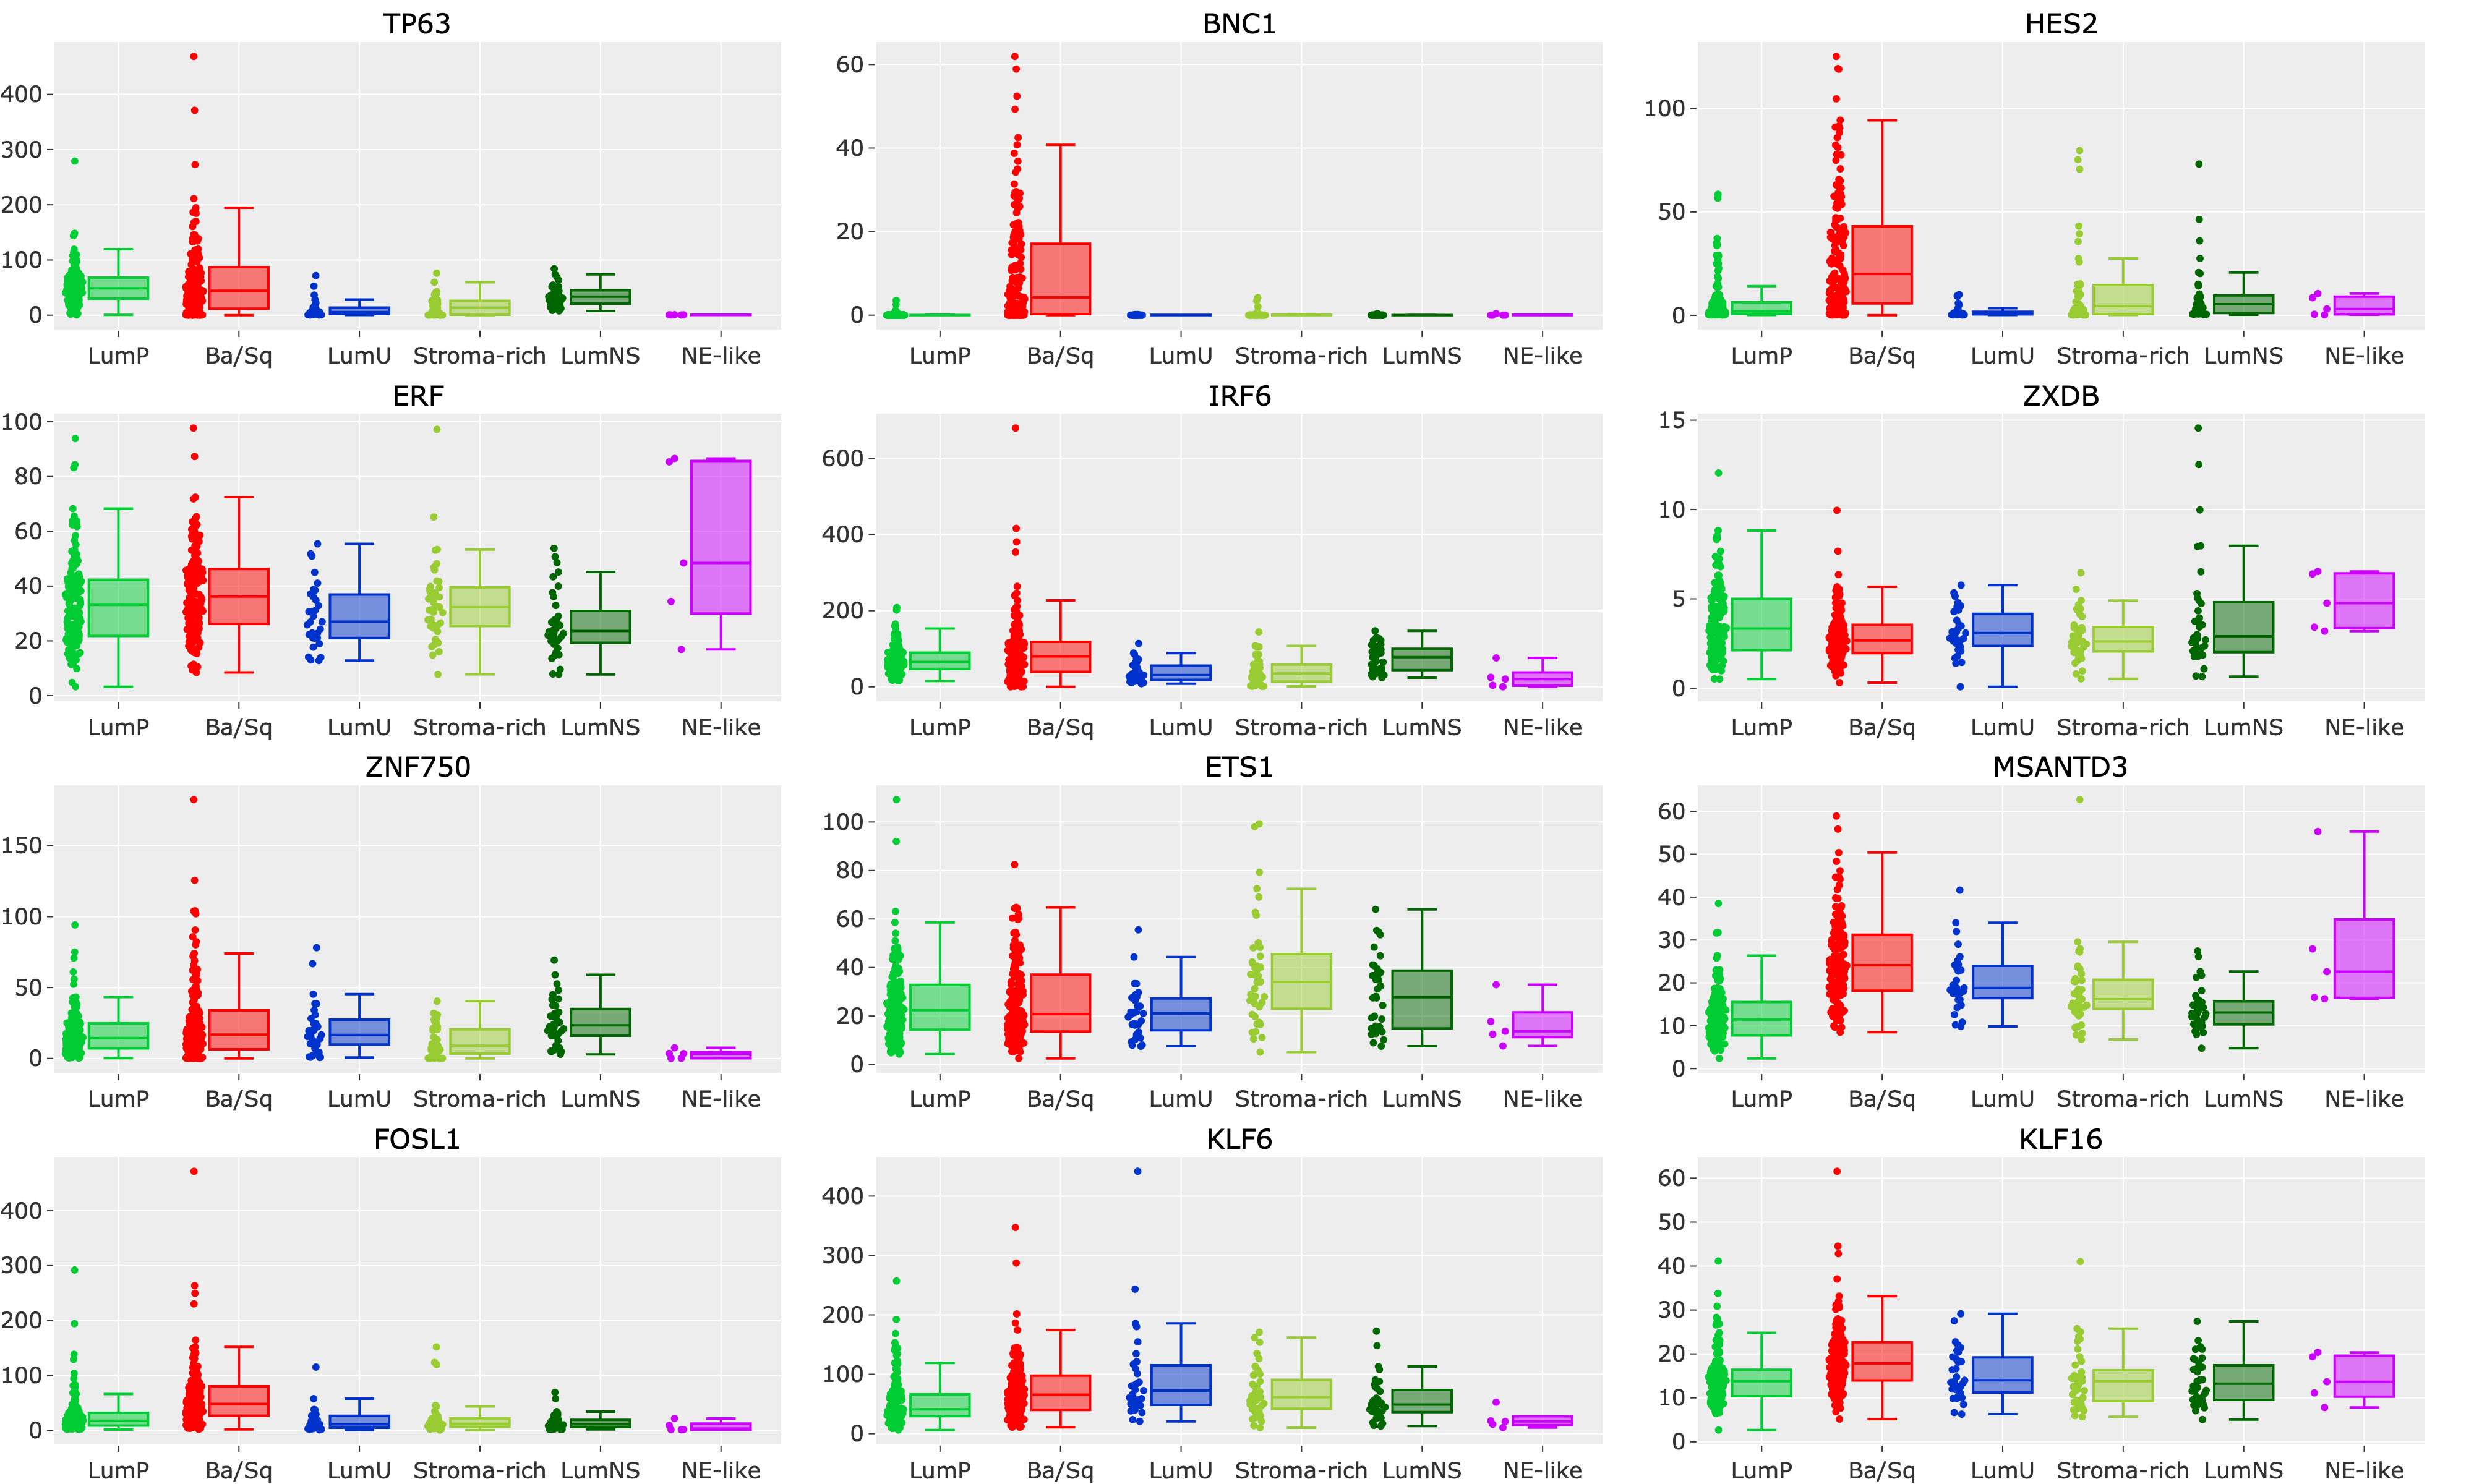
\includegraphics[width=1.0\textwidth,height=1.0\textheight,keepaspectratio]{Sections/Network_I/Resources/selective_pruning/box_plots/consensus_basal.png}
    \caption{Basal}
    \label{fig:ap:box_basal_consensus}
    \end{subfigure}
  \begin{subfigure}[!t]{0.95\textwidth}
      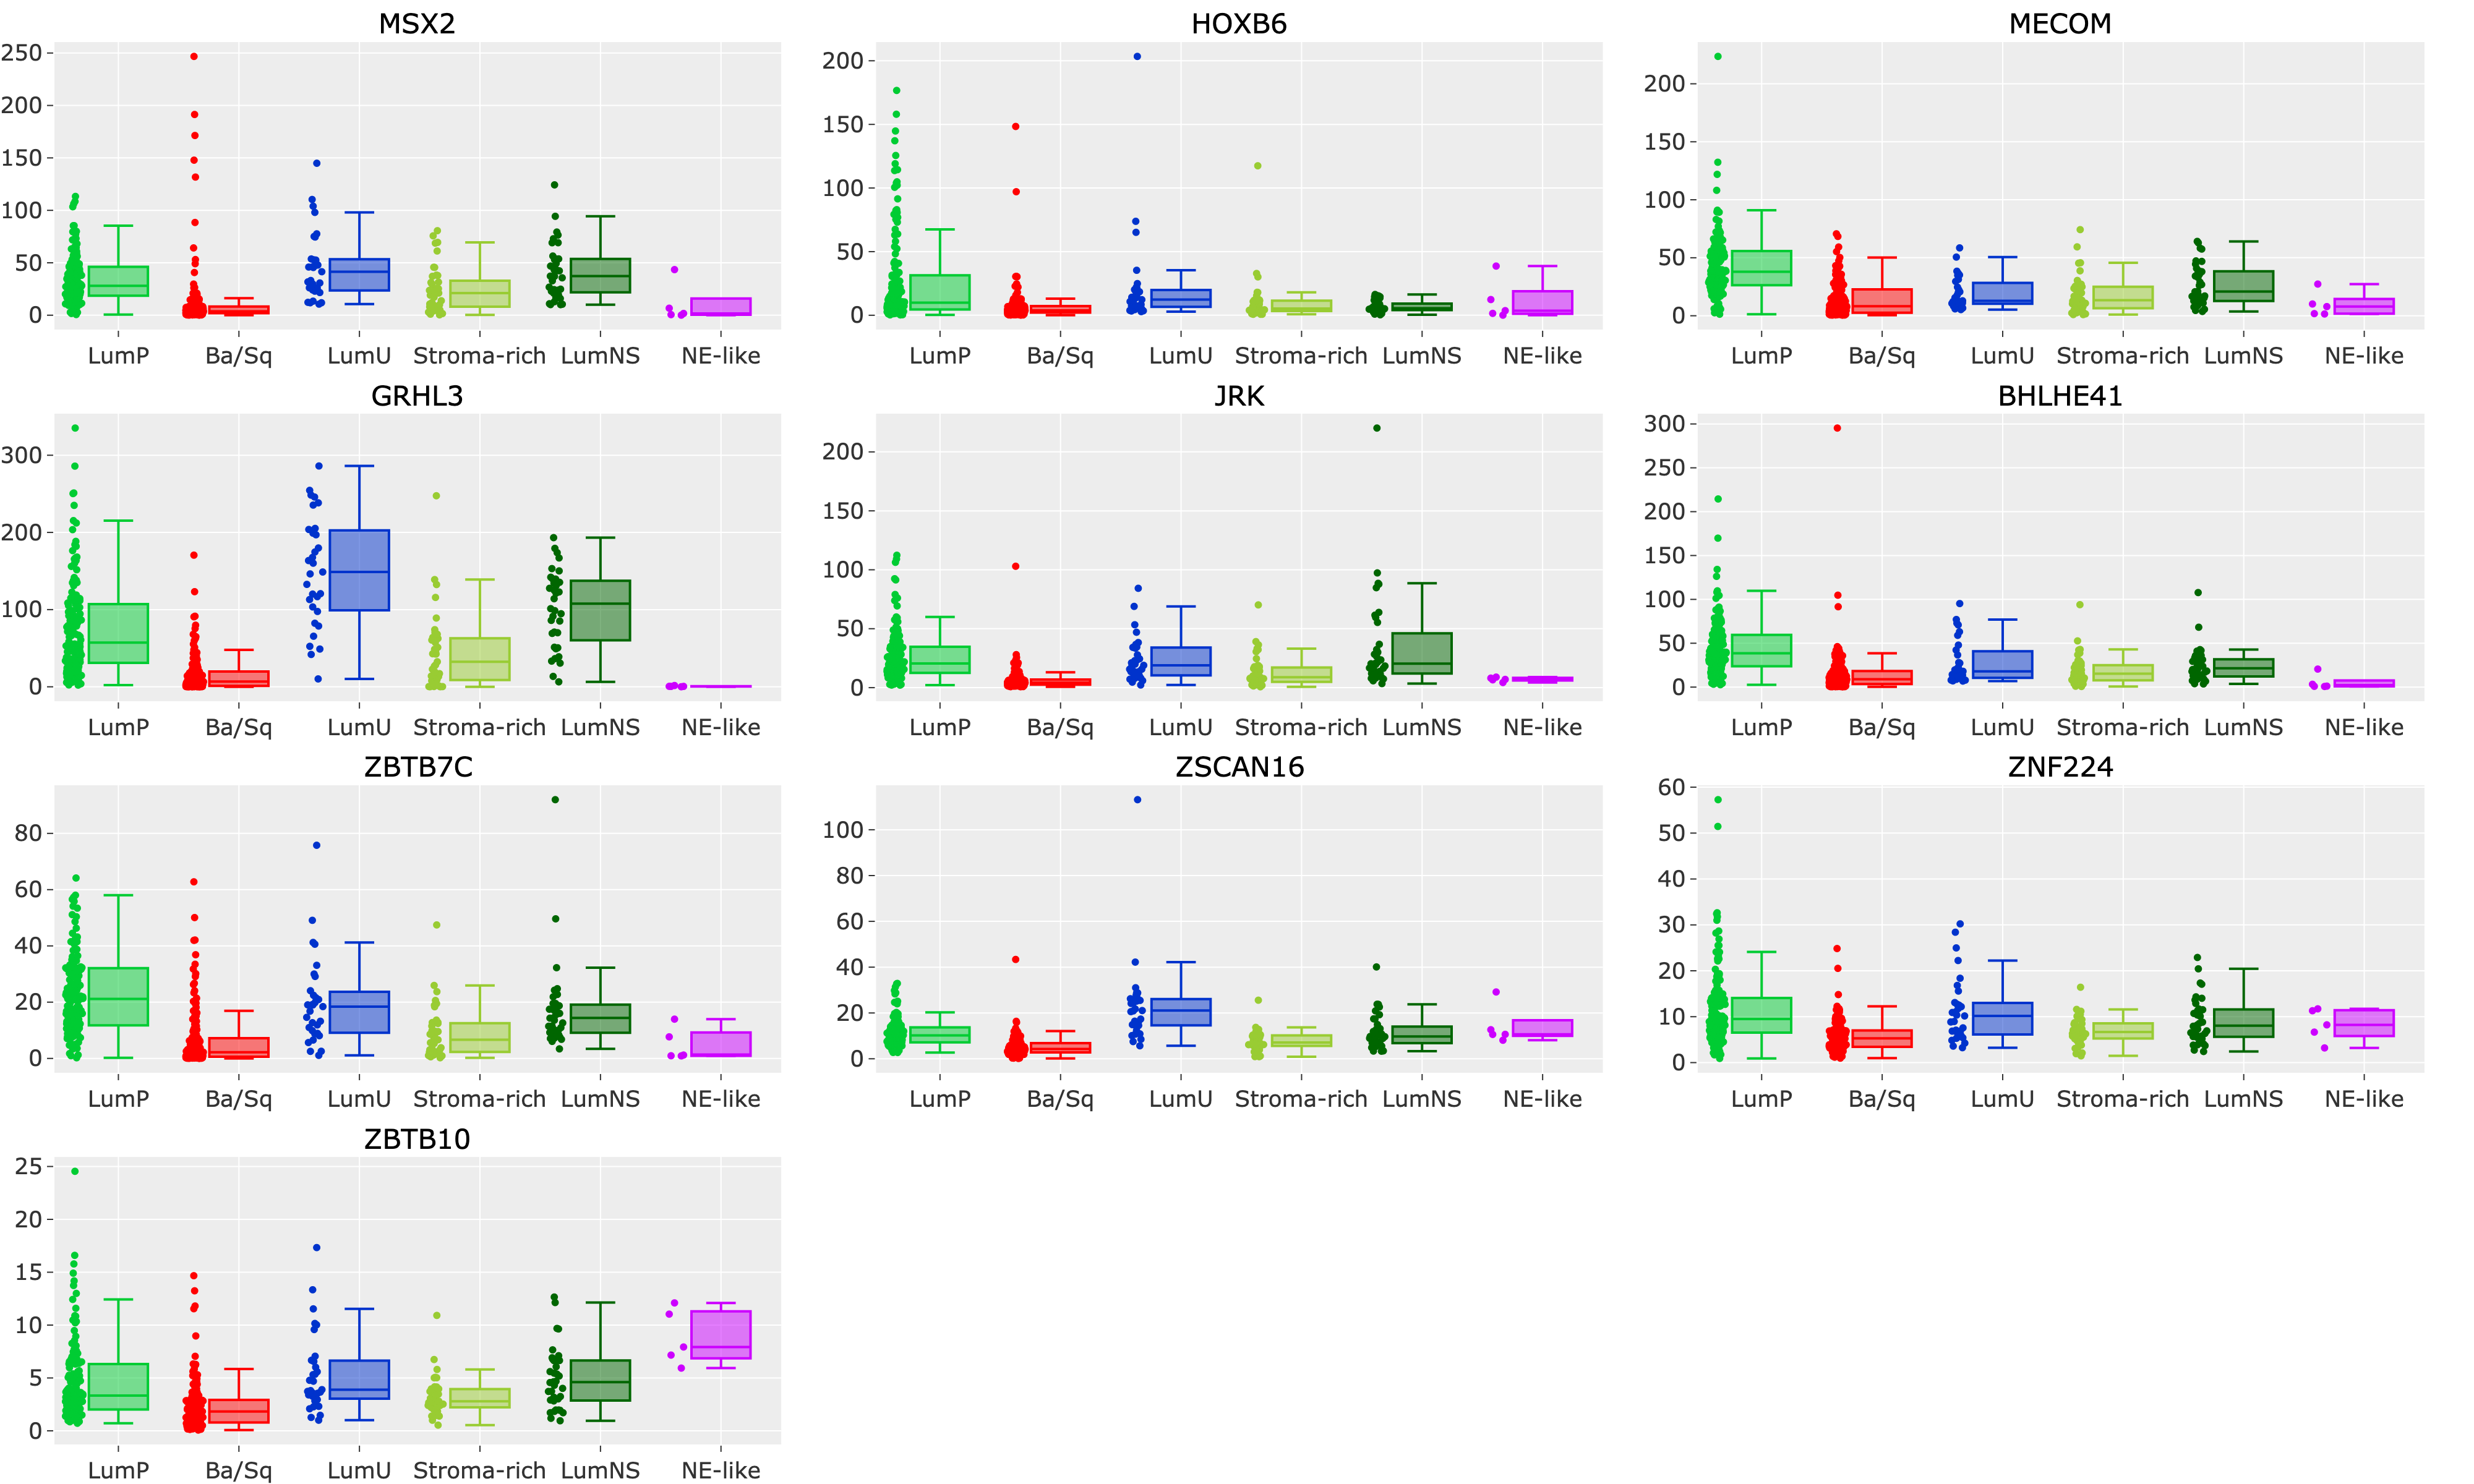
\includegraphics[width=1.0\textwidth,height=1.0\textheight,keepaspectratio]{Sections/Network_I/Resources/selective_pruning/box_plots/consensus_lum.png}
      \caption{Luminal}
      \label{fig:ap:box_luminal_consensus}
  \end{subfigure}
  \caption[Basal and luminal markers of the consensus subtyping]{Box plots showing the TPM spread of the over the consensus MIBC \citet{Kamoun2020-tj}. Supporting the work done in \cref{fig:N_I:box_debdrogram}.}
  \label{fig:ap:box_consensus}
\end{figure}




% Pi-plots for GSEA
\section{Pi-plots for GSEA} \label{s:ap:sel_prun_pi}

This section supports the results from \cref{s:N_I:sel_tfs_subtypes} and it contains the Pi-plots for each of the MIBC subtypes derived from the gene expression of the 98 TF from \cref{s:N_I:sel_tfs}. The method on how the DEA was performed and the Pi-plots generated can be found in \cref{s:lit:dea,s:lit:pi,s:lit:gsea}. Below are some notes on choosing the comparison across the four pi plots:

\paragraph*{Basal 4}

\begin{itemize}
    \item This is the largest basal group (\cref{fig:N_I:sankey_sel_tfs}).
    \item It contains samples that were primarily classified as Ba/Sq by previous stratification methods \citep{Robertson2017-mg,Kamoun2020-tj,Marzouka2018-ge}.
    \item The comparison with the two luminal groups aimed to identify any infiltration trends within Basal 4 and any Ba/Sq-specific markers.
    \item \textbf{Result:} The group has fewer genes in common with the luminal-infiltrated group than expected. Lum 13 exhibits a strong gene expression difference when compared with the large basal group, particularly with values on the negative Y-axis.
\end{itemize}
    
\paragraph*{Luminal 13 (Lum 13)}

\begin{itemize}
    \item This is the largest luminal group (\cref{fig:N_I:sankey_sel_tfs}).
    \item It consists of most of the luminal samples \citep{Robertson2017-mg,Kamoun2020-tj,Marzouka2018-ge}.
    \item The comparison with Basal 5 and Basal 4 was intended to highlight the luminal markers specific to this group.
    \item \textbf{Result:} In \cref{fig:ap:pi_lum}, Lum 13 exhibits a strong gene expression difference, especially when compared with Basal 5. The two basal groups show some common markers.
\end{itemize}

\paragraph*{Mes 3}

\begin{itemize}
    \item This group consists of samples classified as Mes-like by the Lund classifier \citep{Marzouka2018-ge}.
    \item The comparison with Lum 13 and Lum 12 aimed to identify any basal markers specific to Mes 3.
    \item \textbf{Result:} The Pi plot in \cref{fig:ap:mes_like} shows a strong difference between the luminal groups and Mes-like, which is expected given that some of the samples were previously classified as basal. The luminal groups share several genes.
\end{itemize}

\paragraph*{Luminal 12 (Lum 12)}
 
\begin{itemize}
    \item This group contains a large share of samples previously classified as luminal infiltrated \cite{Robertson2017-mg,Kamoun2020-tj}.
    \item The comparison with Basal 5 emphasizes the luminal markers specific to Lum 13, while the comparison with Basal 4 checks for shared immune genes.
    \item \textbf{Result:} The group exhibits a strong gene expression difference with the basal groups. As seen in \cref{fig:ap:lumInf}, there are not many immune markers shared between Basal 4 and Lum 13.
\end{itemize}


\begin{figure}[H]
    \centering
    \begin{subfigure}[!t]{1.0\linewidth}
        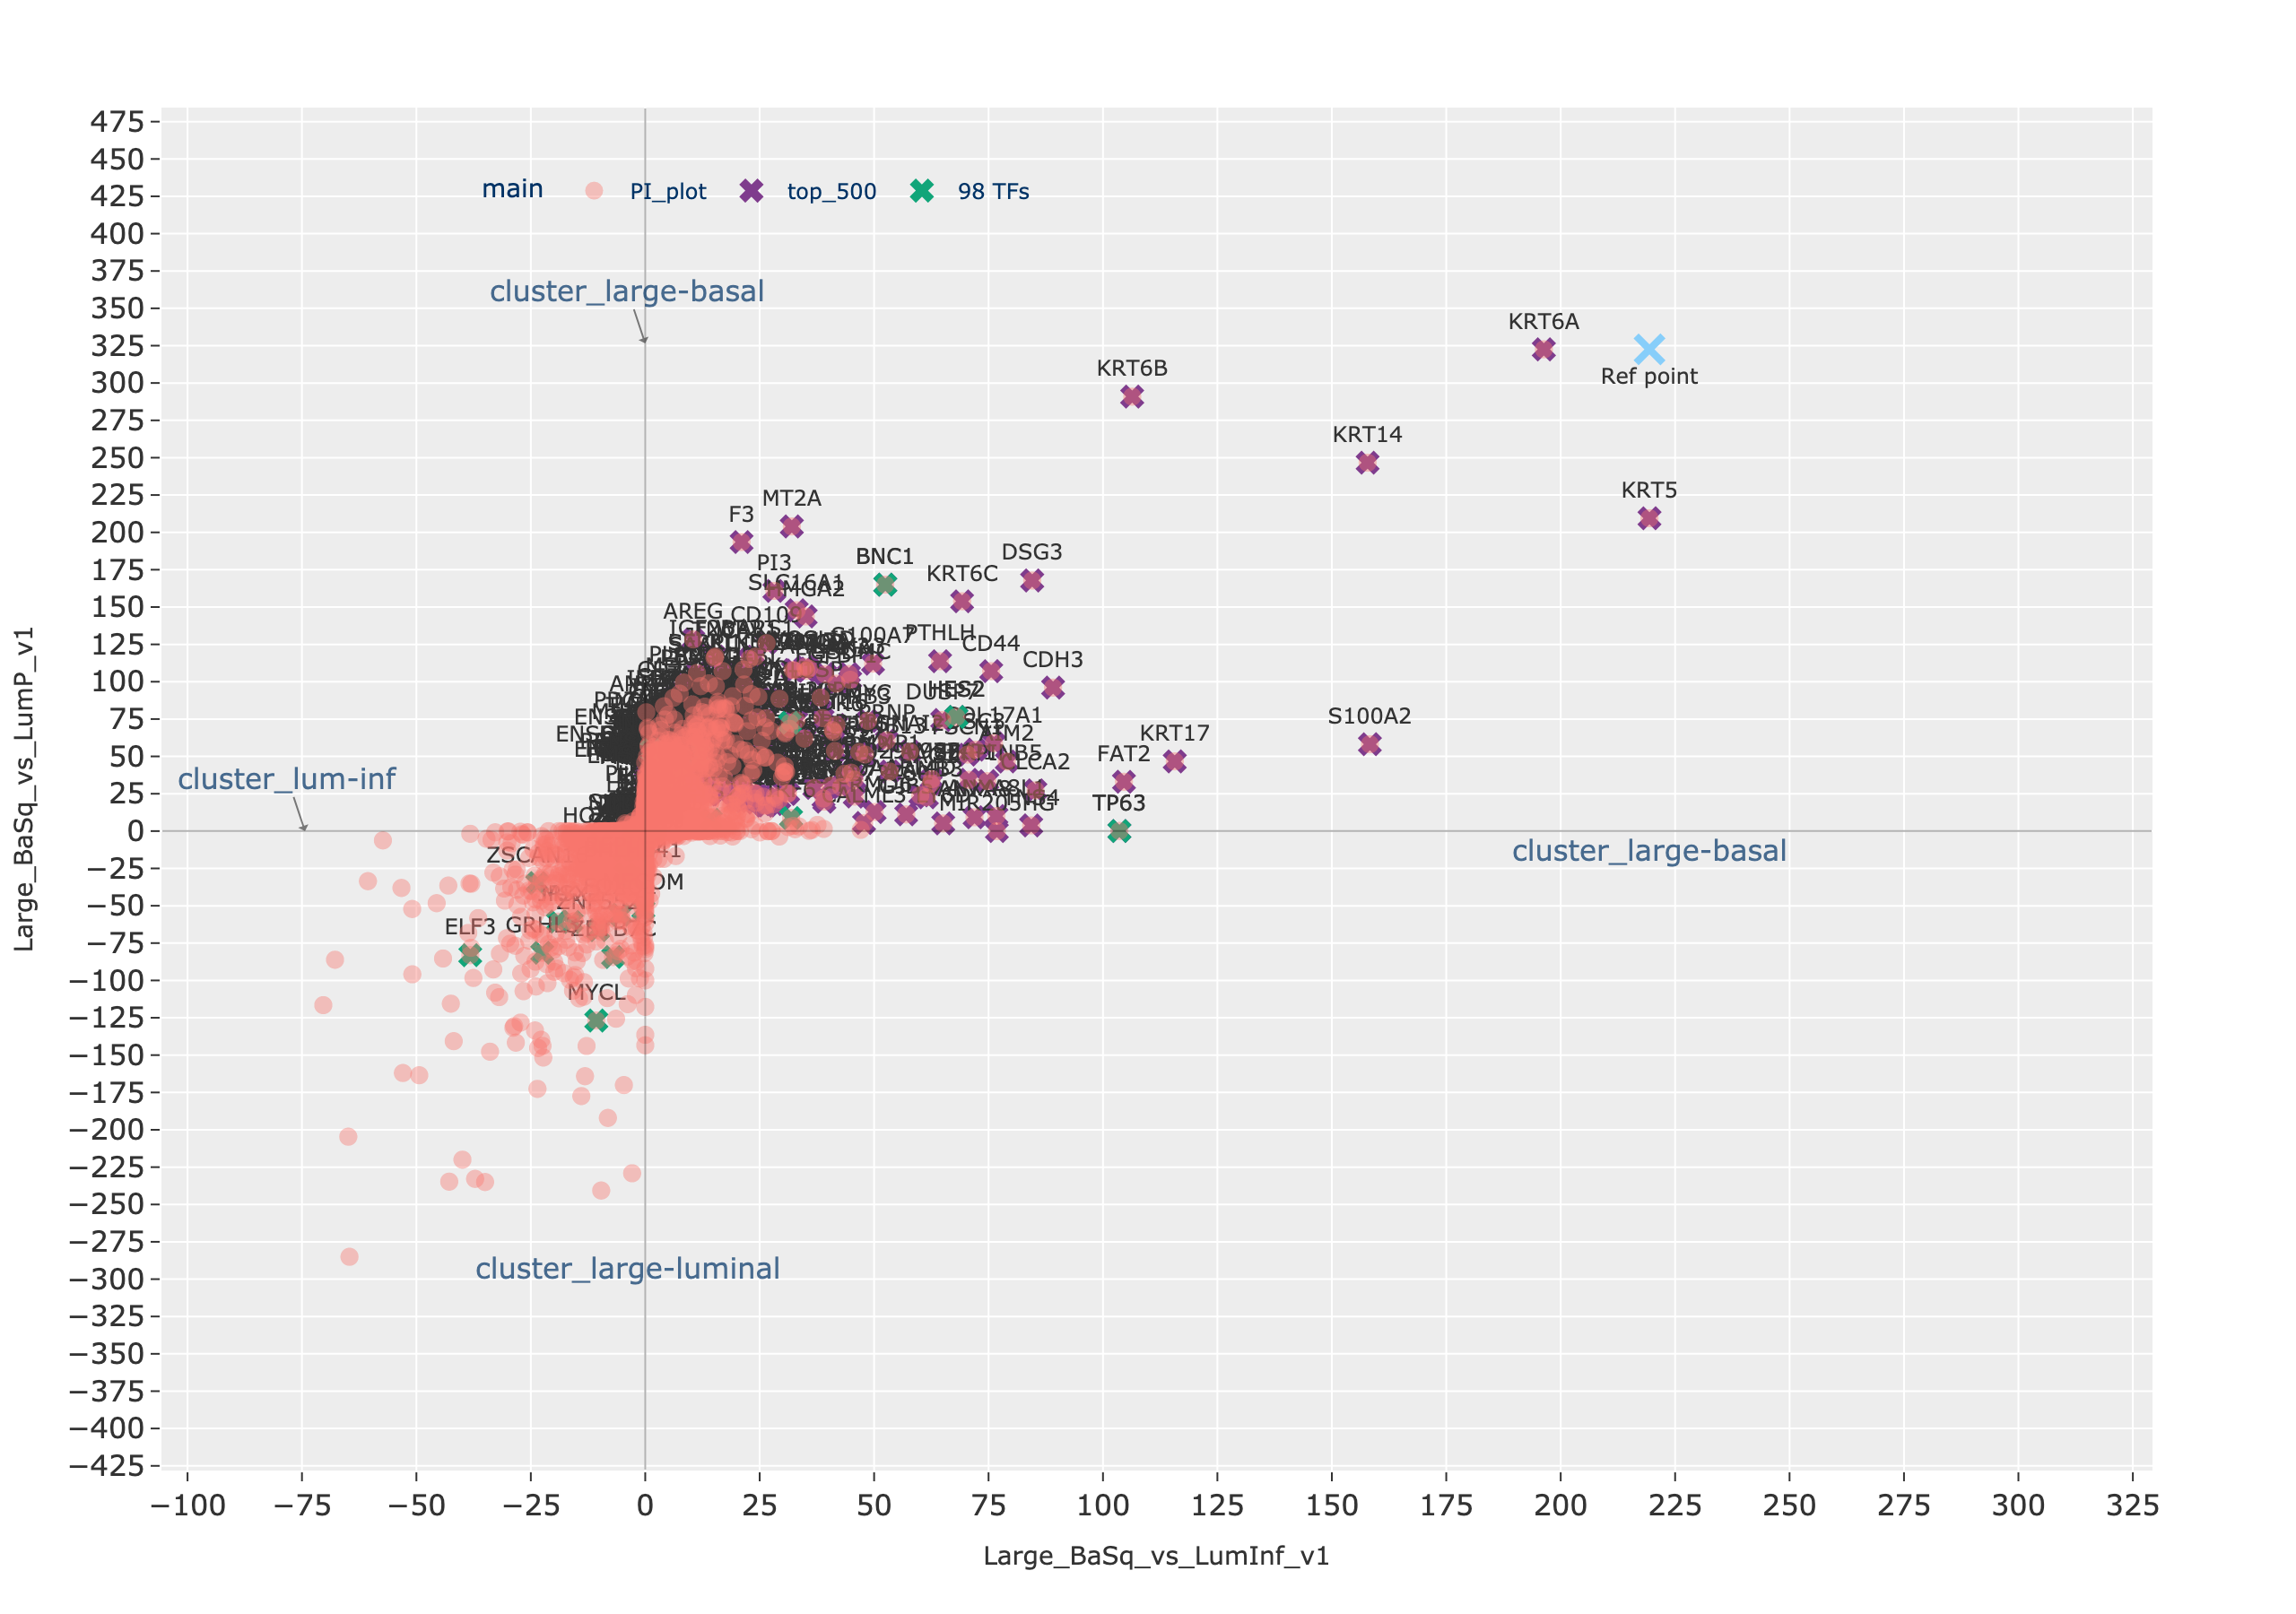
\includegraphics[width=\textwidth,keepaspectratio]{Sections/Network_I/Resources/selective_pruning/pi_gsea/pi_largeBasal.png}
        \caption{Basal 4 - the largest basal group}
        \label{fig:ap:pi_basal}
    \end{subfigure}
    \begin{subfigure}[!t]{1.0\textwidth}
        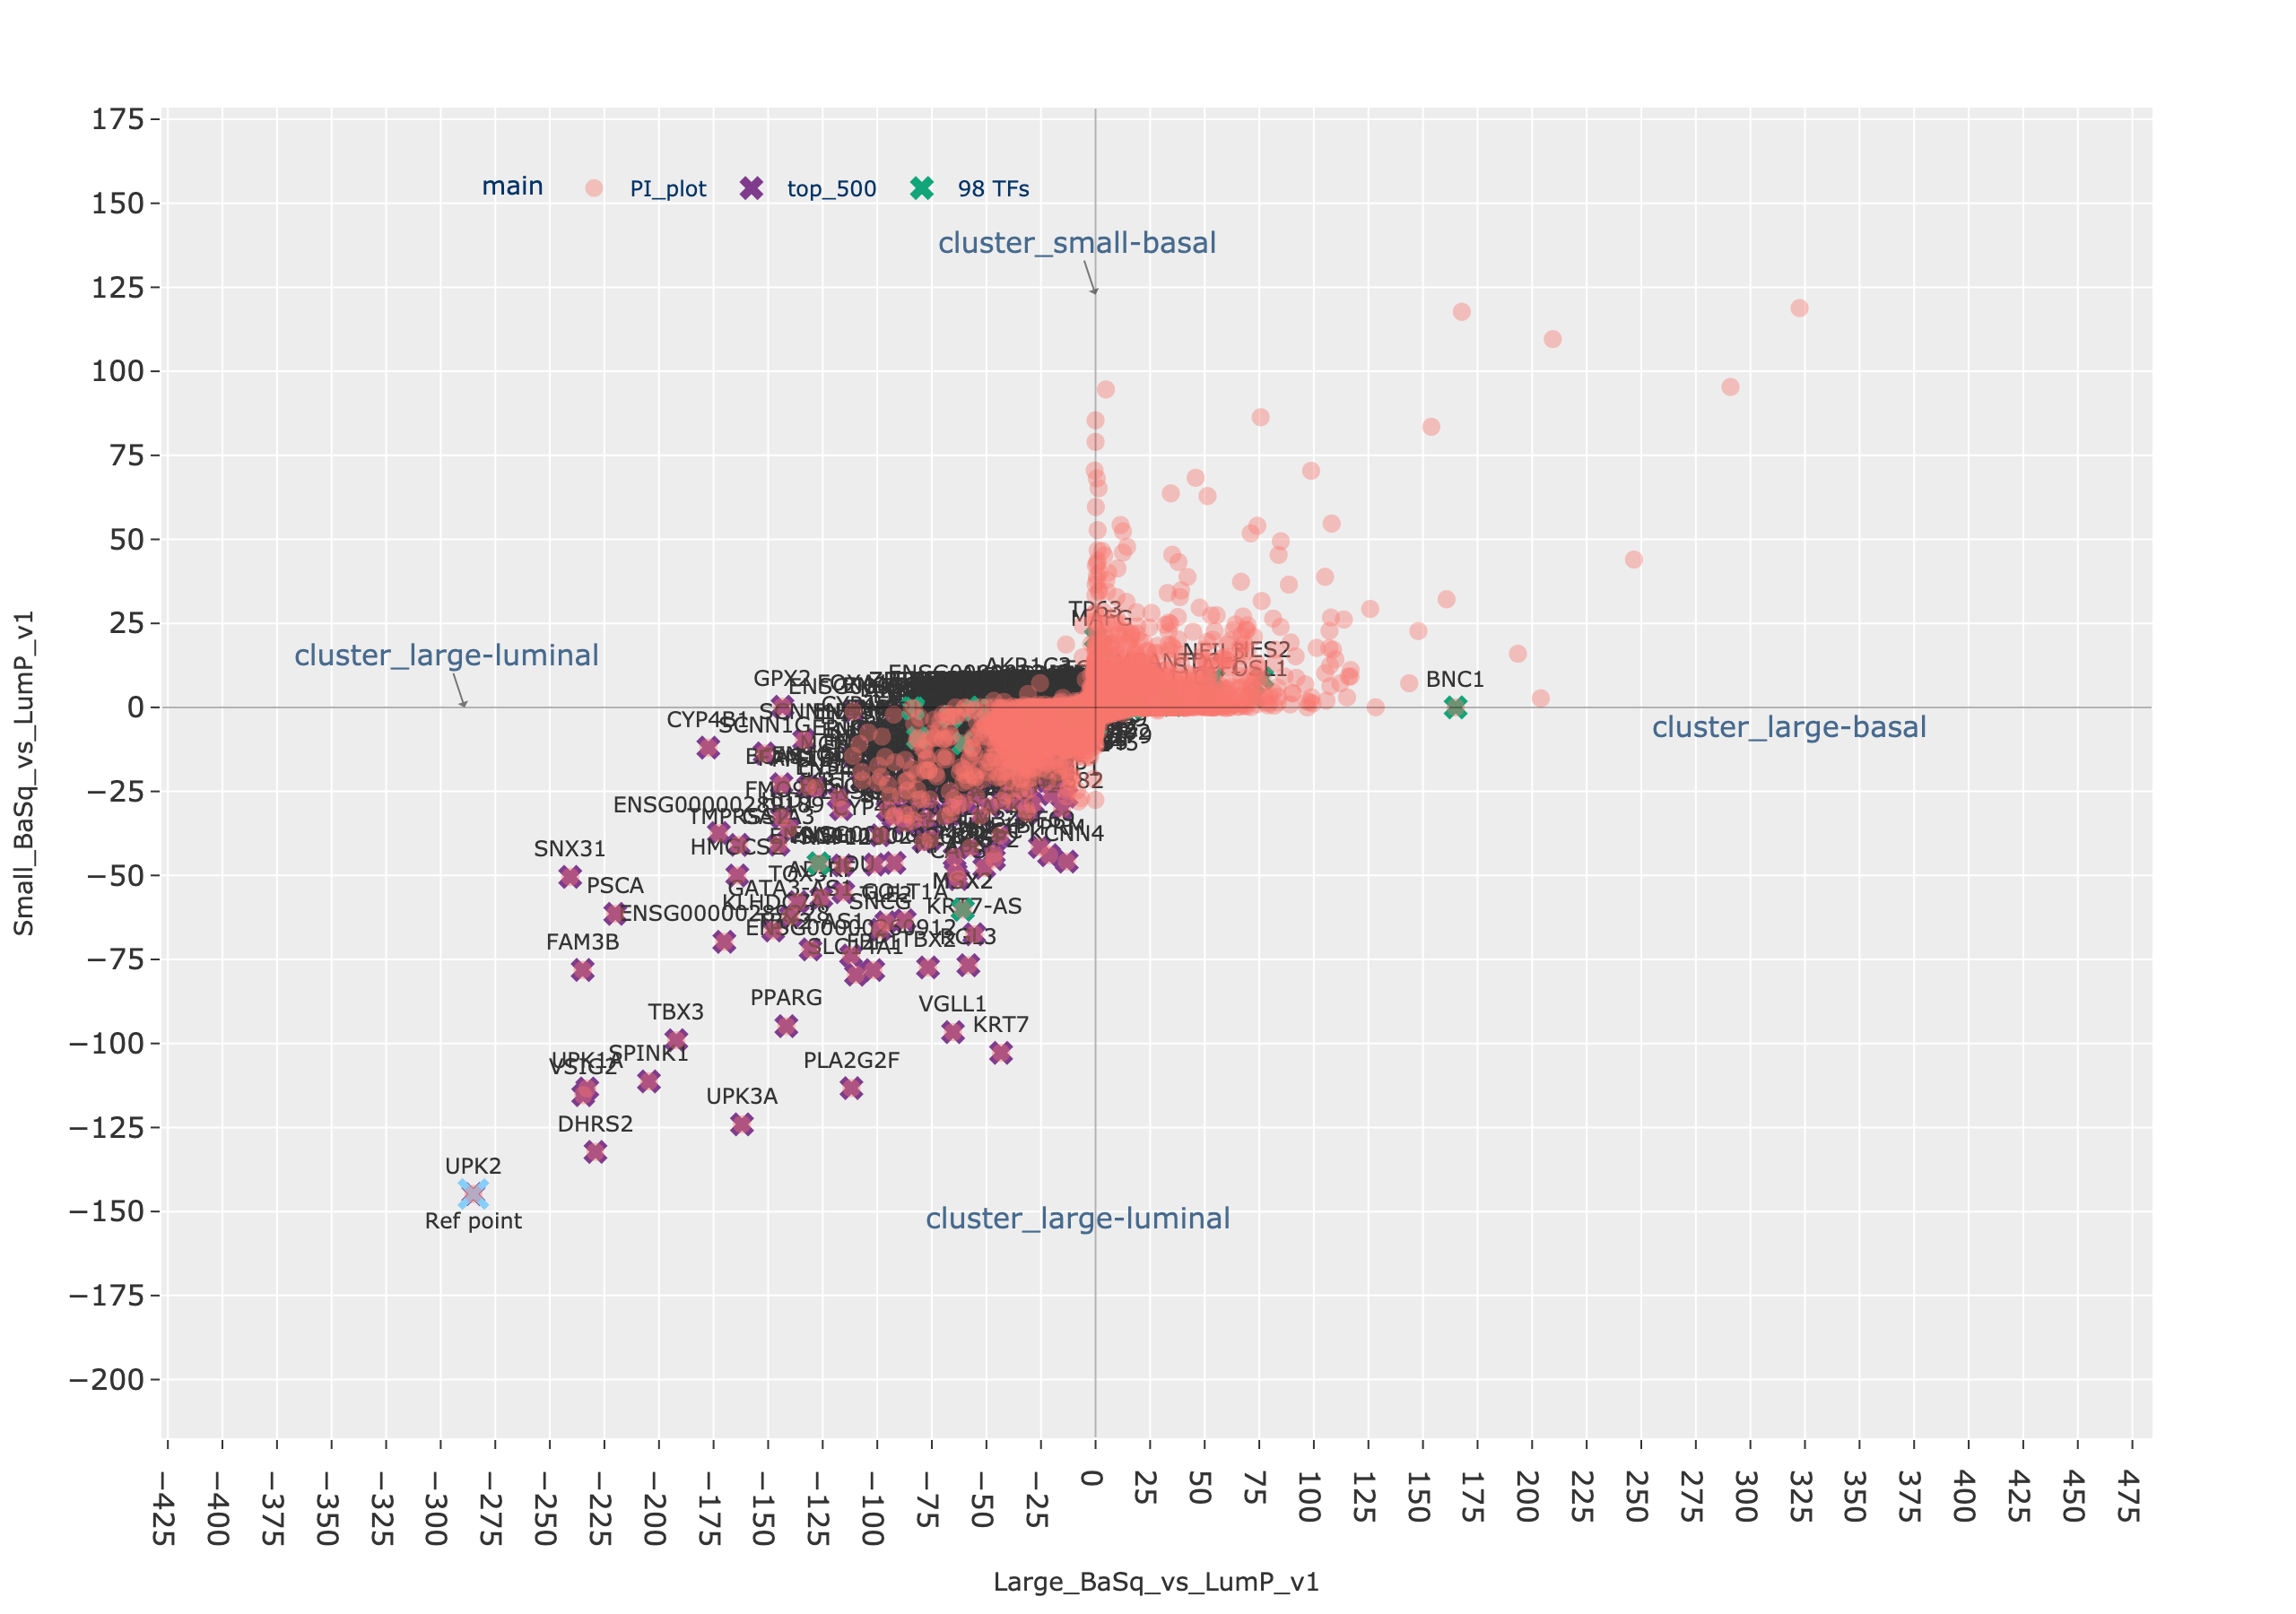
\includegraphics[width=\textwidth,keepaspectratio]{Sections/Network_I/Resources/selective_pruning/pi_gsea/pi_largeLuminal.png}
        \caption{Lum 13 - biggest luminal group}
        \label{fig:ap:pi_lum}
    \end{subfigure}
    \caption[Basal 4 and Lum 13 pi plots]{Pi plots Basal 4 and Lum 13 from \cref{s:N_I:sel_tfs_subtypes} which were used used to rank the genes for the GSEA in \cref{s:ap:sel_tfs_gsea_reactome}.}
    \label{fig:ap:pi_other_values_I}
\end{figure}

\begin{figure}[!h]
    \centering
    \begin{subfigure}[!t]{1.0\textwidth}
        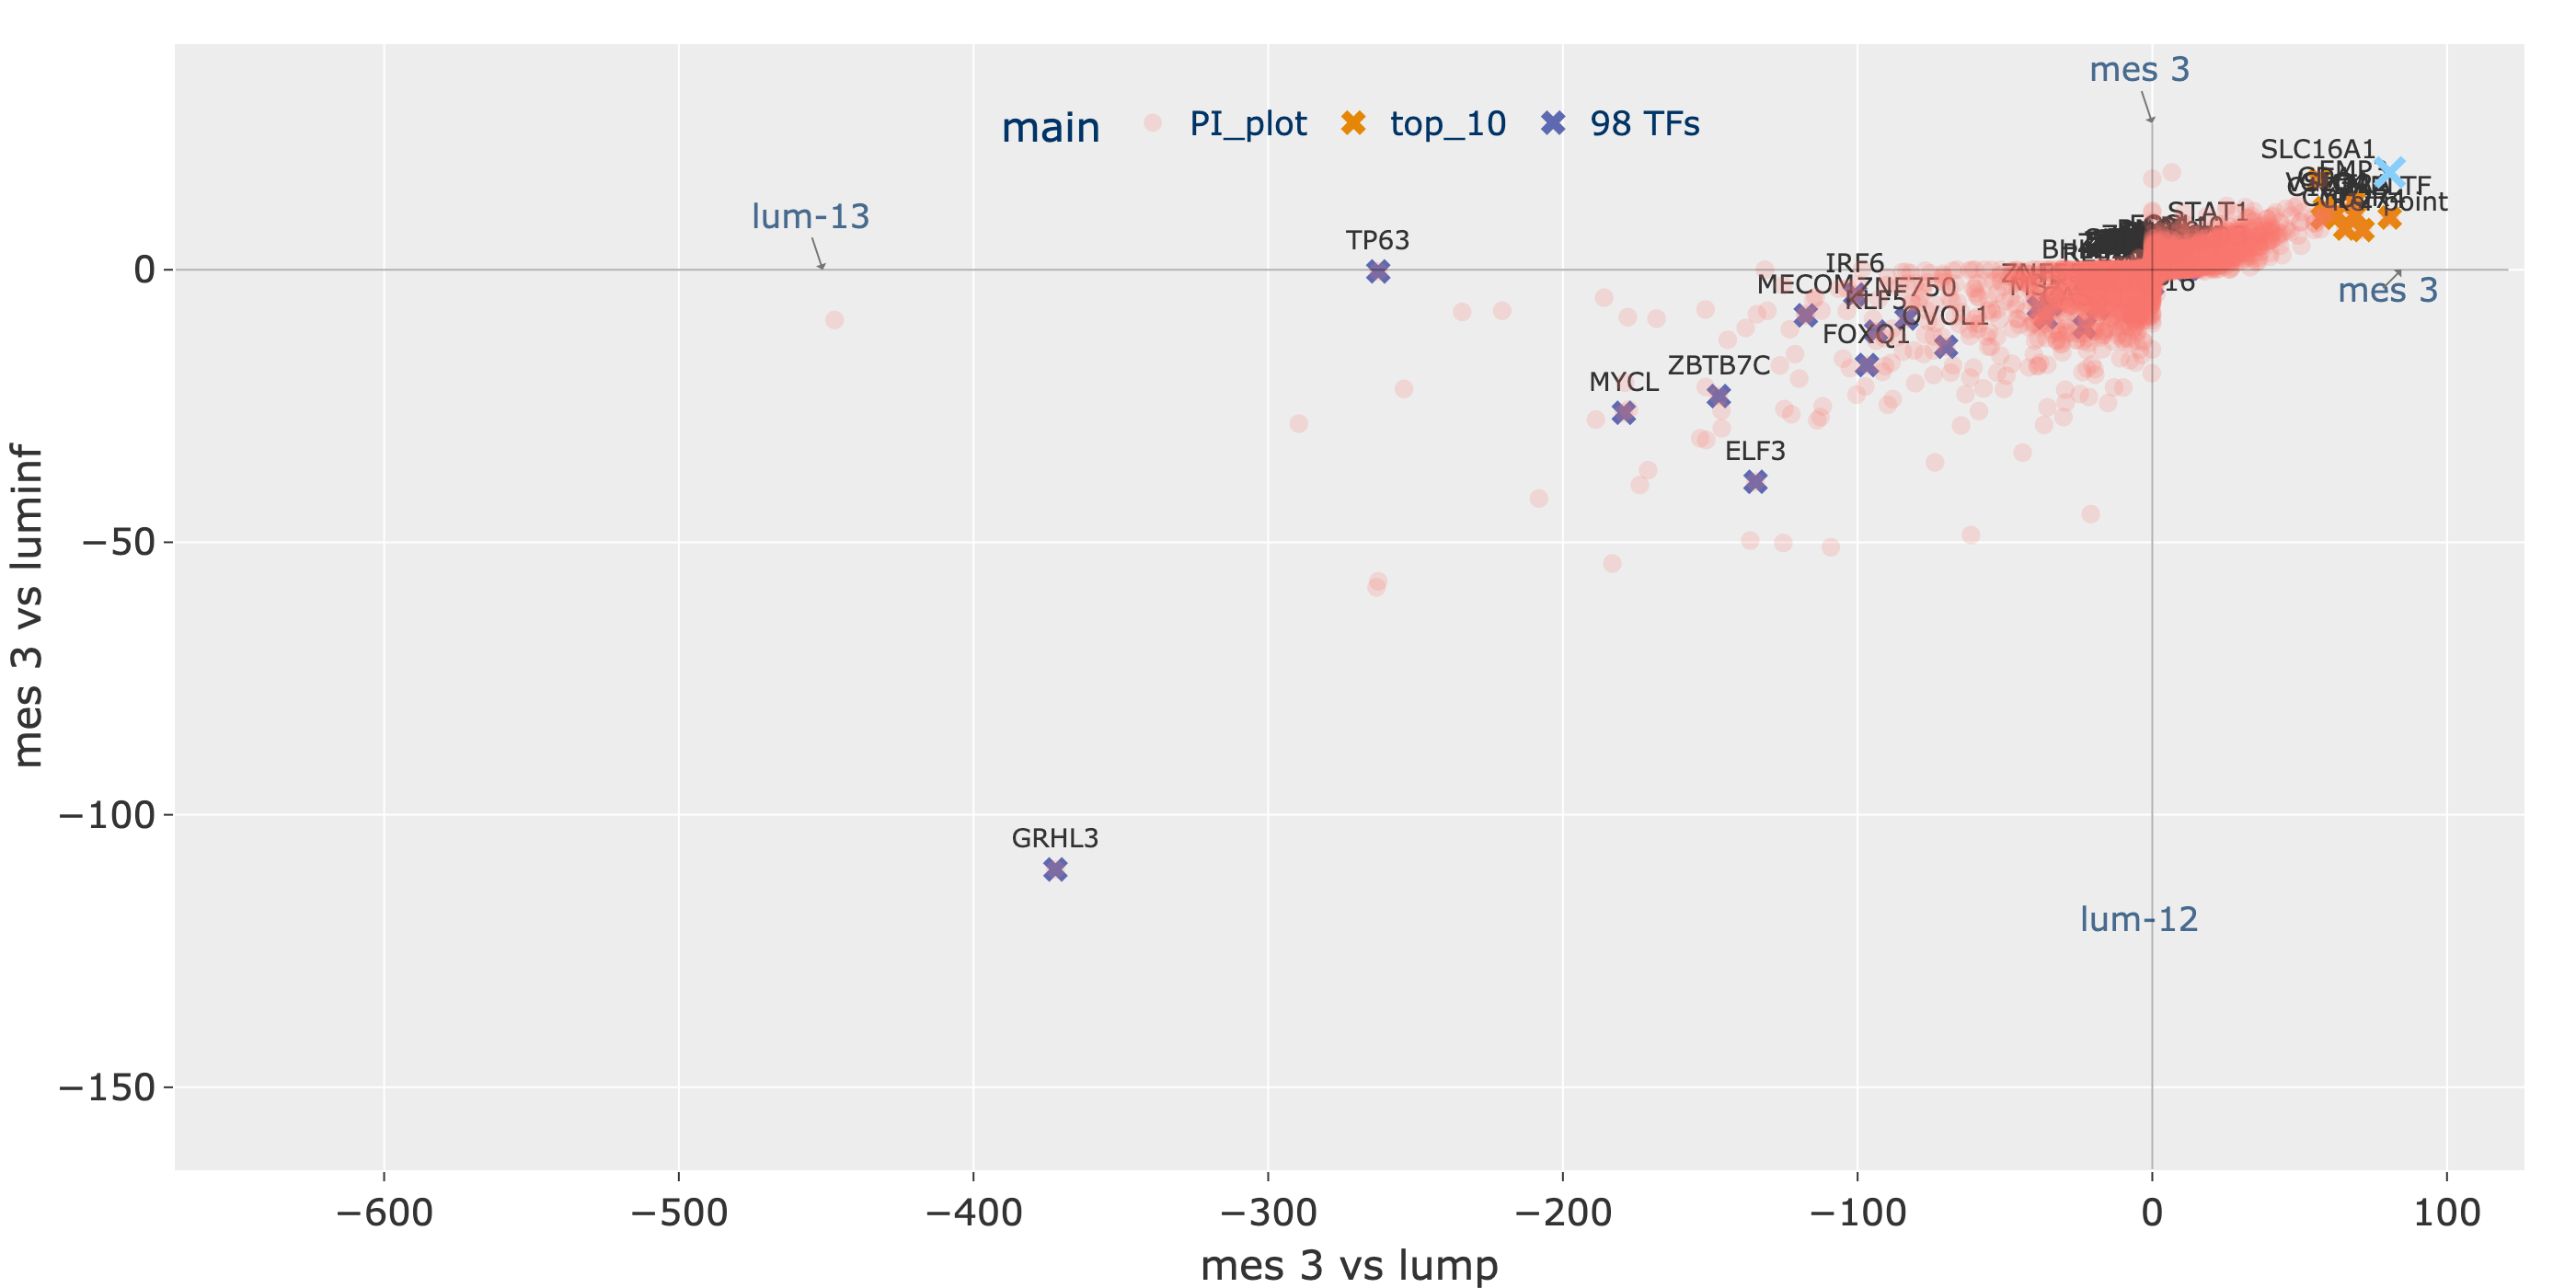
\includegraphics[width=\textwidth,keepaspectratio]{Sections/Network_I/Resources/selective_pruning/pi_gsea/pi_mesLike.png}
        \caption{Mes 3}
        \label{fig:ap:mes_like}
    \end{subfigure}
    \begin{subfigure}[!t]{1.0\textwidth}
        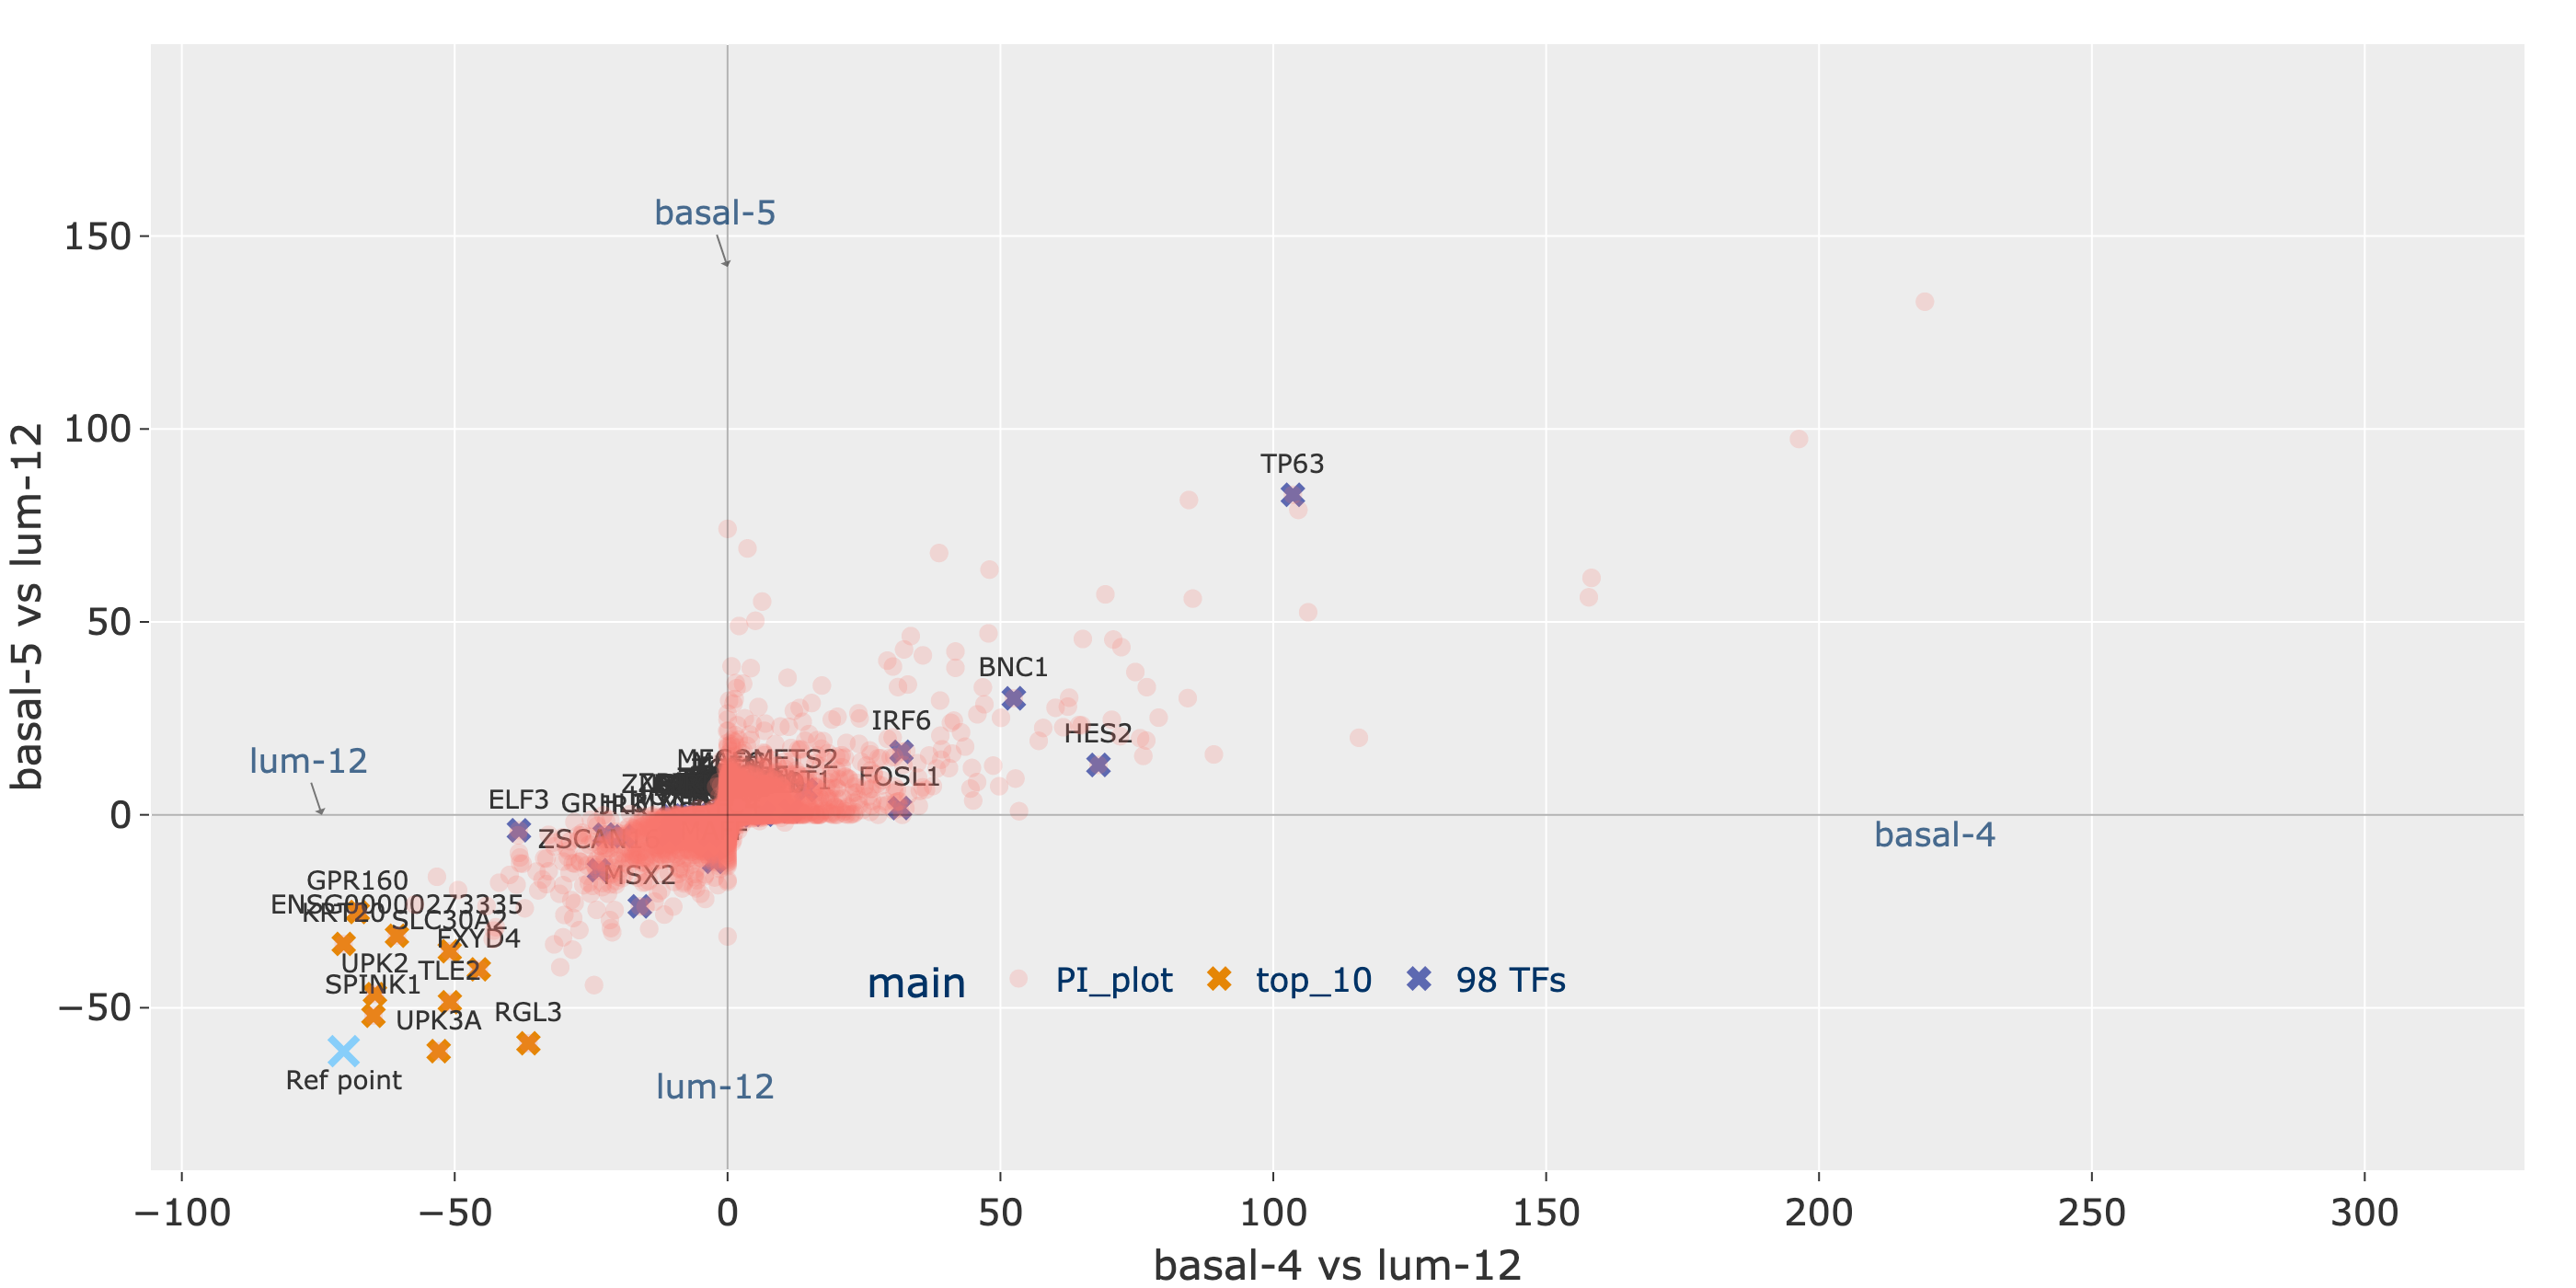
\includegraphics[width=\textwidth,keepaspectratio]{Sections/Network_I/Resources/selective_pruning/pi_gsea/pi_lumInf.png}
        \caption{Luminal 12 - or luminal infiltrated}
        \label{fig:ap:lumInf}
    \end{subfigure} 
    \caption[Mes-3 and Lum 12 pi plots]{Pi plots Mes 3 and Lum 12 from \cref{s:N_I:sel_tfs_subtypes} which were used used to rank the genes for the GSEA in \cref{s:ap:sel_tfs_gsea_reactome}.}
    \label{fig:ap:pi_other_values_II}
\end{figure}

\newpage


% GSEA plots
\section{GSEA plots top 10 - Reactome} \label{s:ap:sel_tfs_gsea_reactome}

This section supports the results presented in \cref{s:N_I:sel_tfs_mibc}, where the five subtypes were derived using the gene expression of the 98 TF identified through selective edge pruning, as discussed in \cref{s:N_I:sel_tfs}. The Pi plots used to rank the data can be seen in \cref{s:ap:sel_prun_pi}. This section contains the GSEA results with the top 10 terms for each group.


\begin{figure}[!htb]
    \centering
    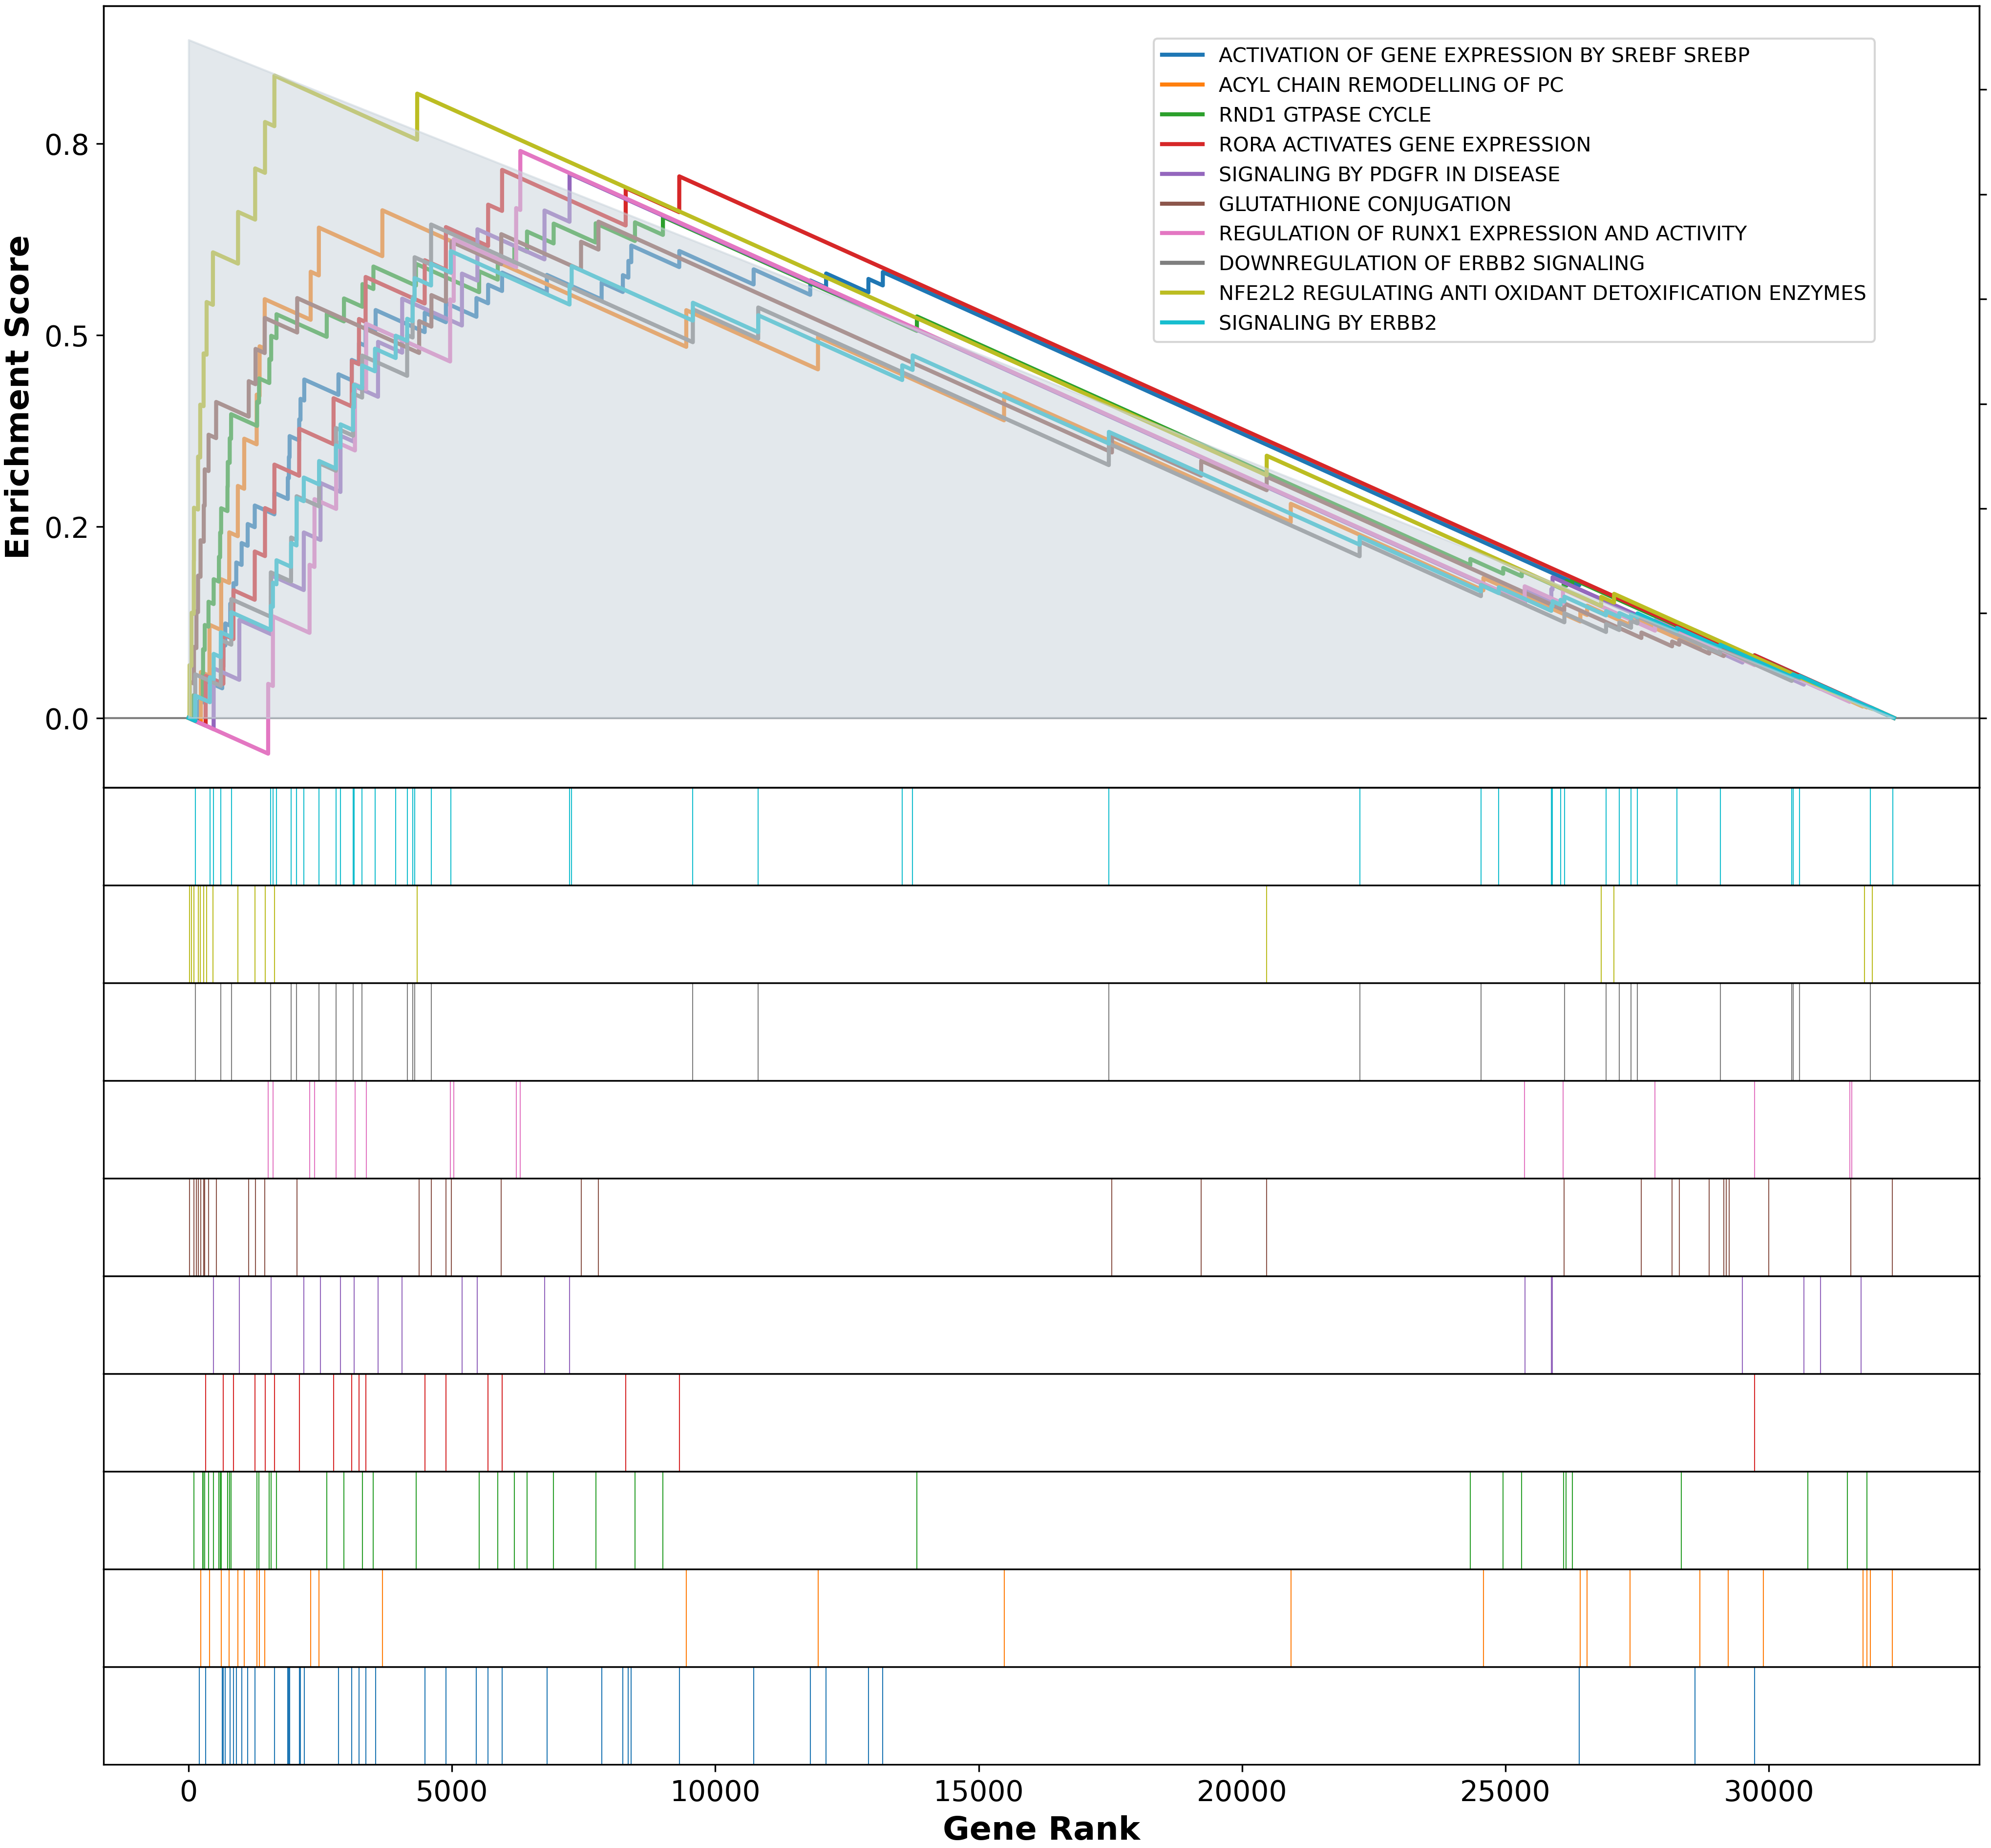
\includegraphics[width=\textwidth,keepaspectratio]{Sections/Network_I/Resources/selective_pruning/gsea/smallBasal_10_top_manTerms.png}
    \caption[Basal 5: GSEA top 10 Reactome terms]{Top 10 GSEA terms with Reactome database for the Basal 5 group. Results interpretation in \cref{s:N_I:sel_tfs_mibc,s:ap:sel_prun_pi}.}
    \label{fig:ap:gsea_smallBasal}
\end{figure}


\begin{figure}[!htb]
    \centering
    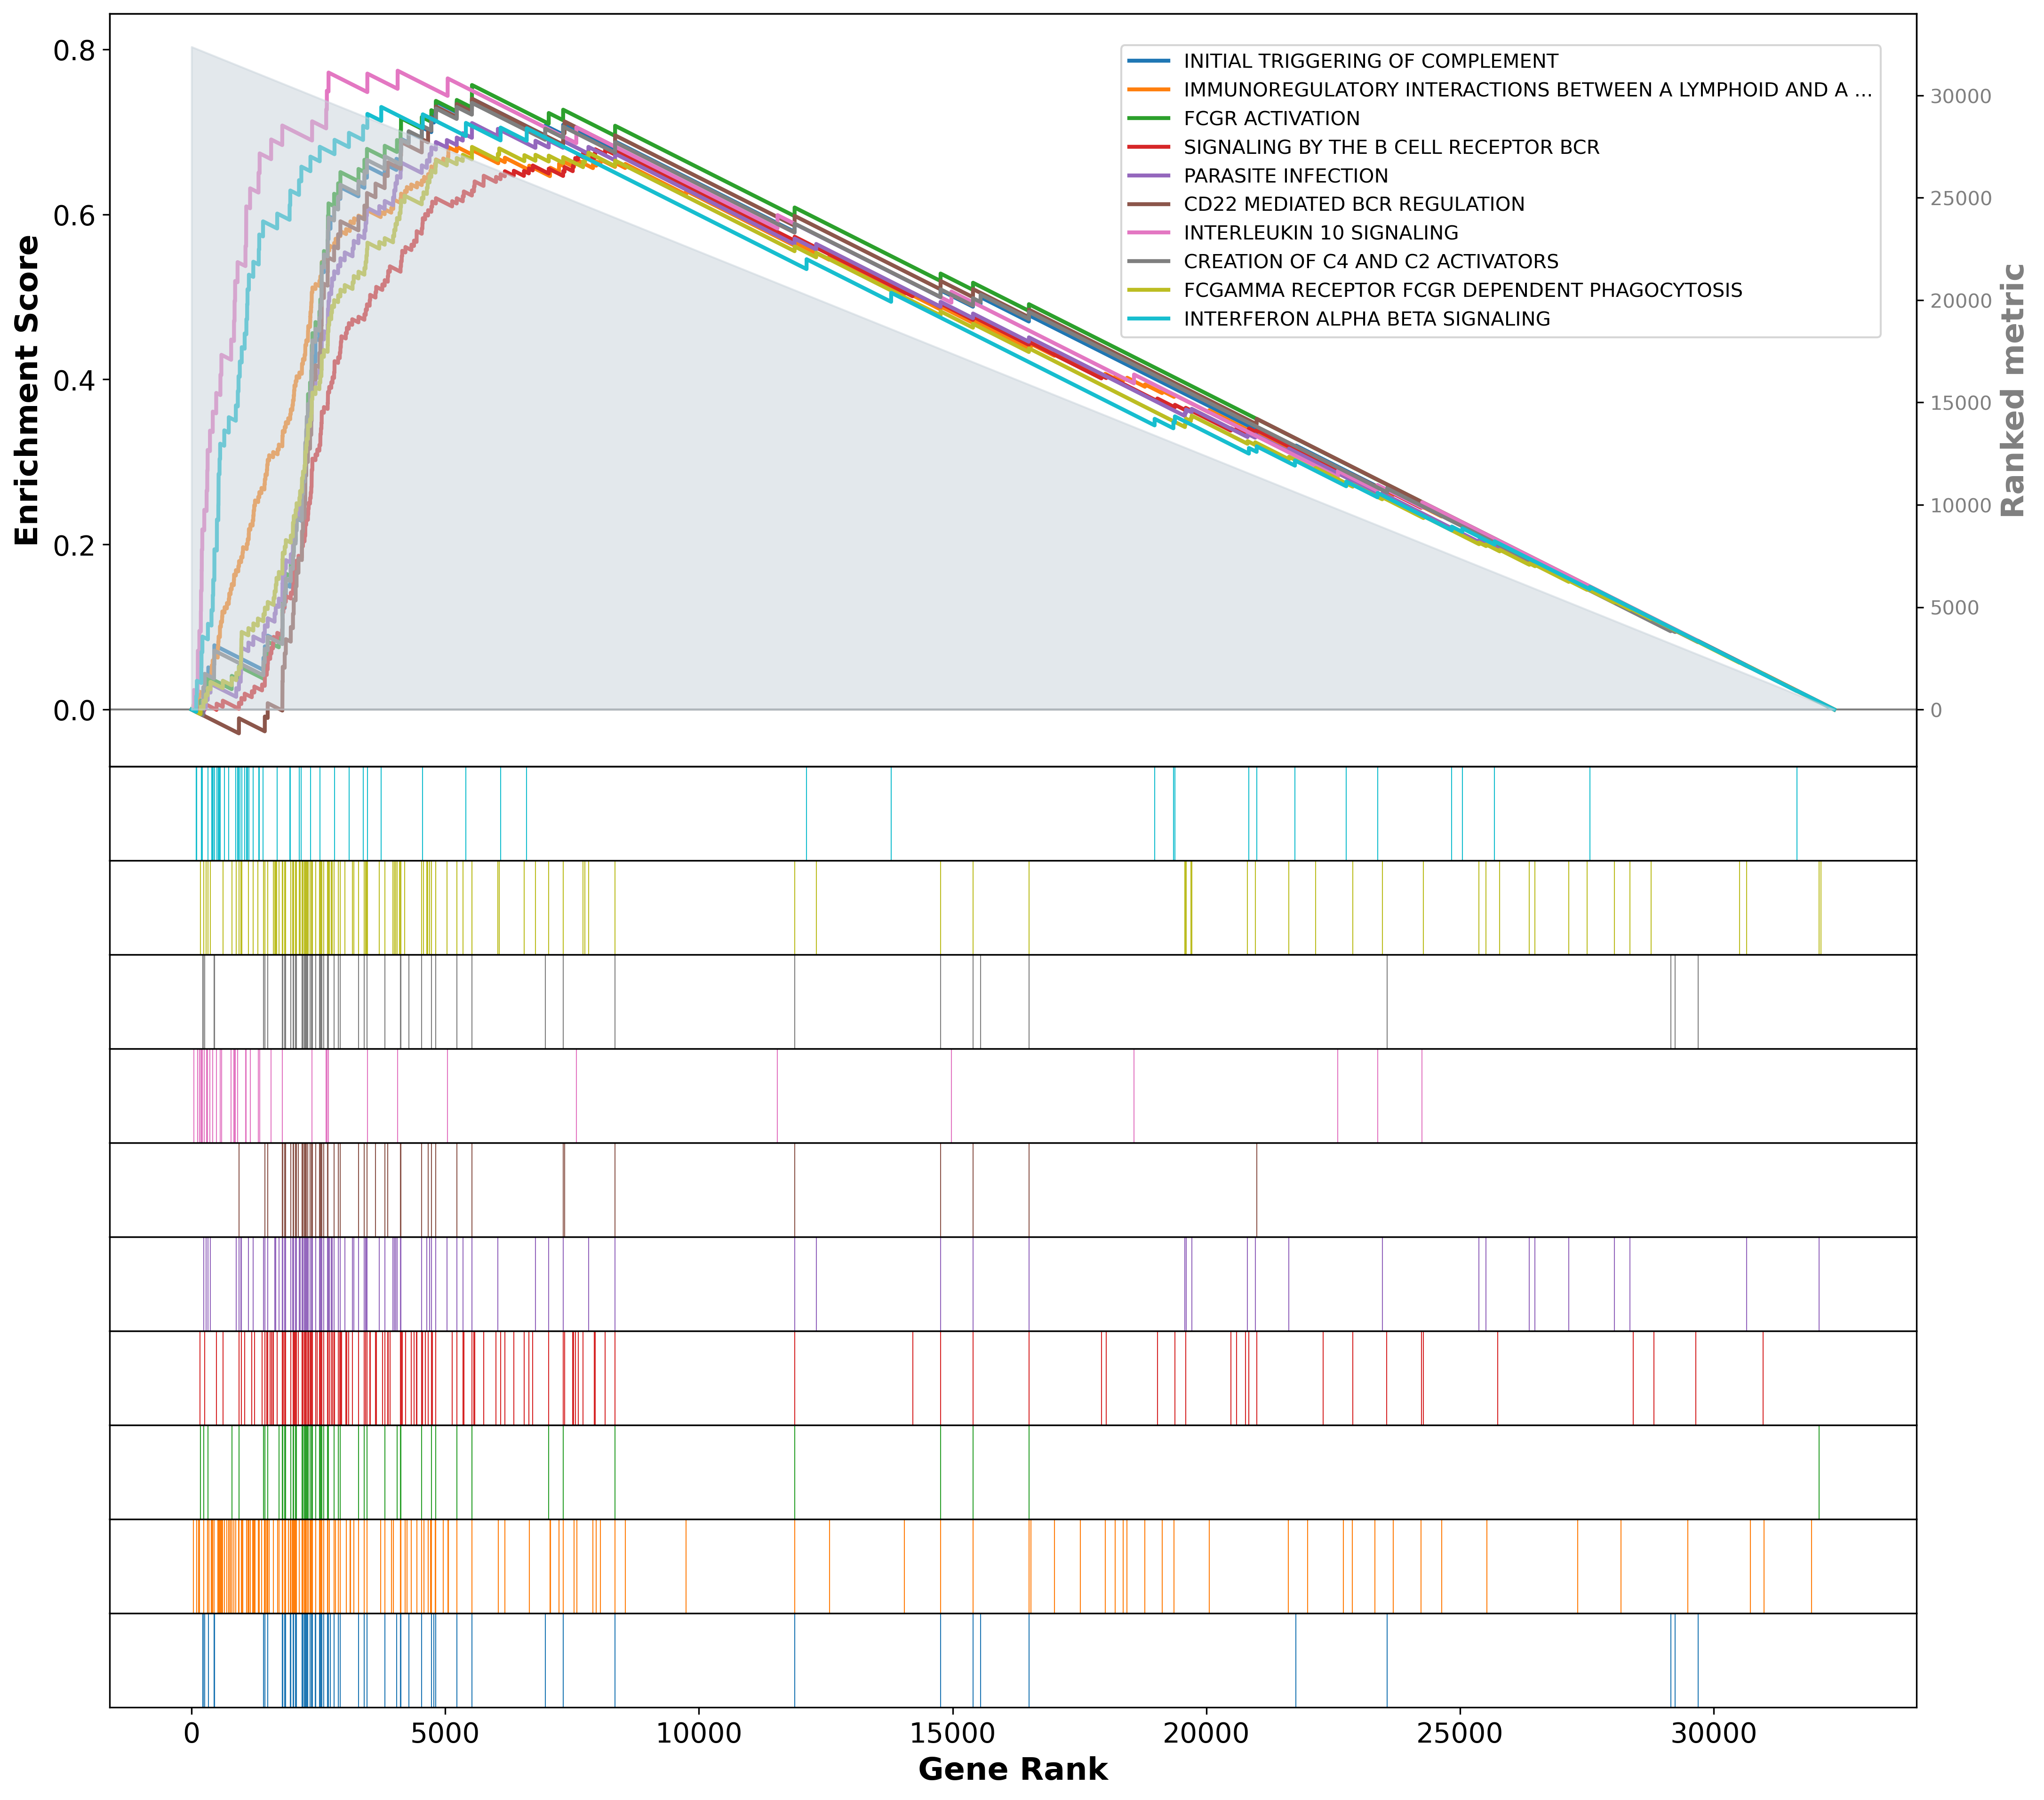
\includegraphics[width=\textwidth,keepaspectratio]{Sections/Network_I/Resources/selective_pruning/gsea/largeBasal_10_top_manTerms.png}
    \caption[Basal 4: GSEA top 10 Reactome terms]{Top 10 GSEA terms with Reactome database for the Basal 4 group. Results interpretation in \cref{s:N_I:sel_tfs_mibc,s:ap:sel_prun_pi}.}
    \label{fig:ap:gsea_largeBasal}
\end{figure}

\begin{figure}[!htb]
    \centering
    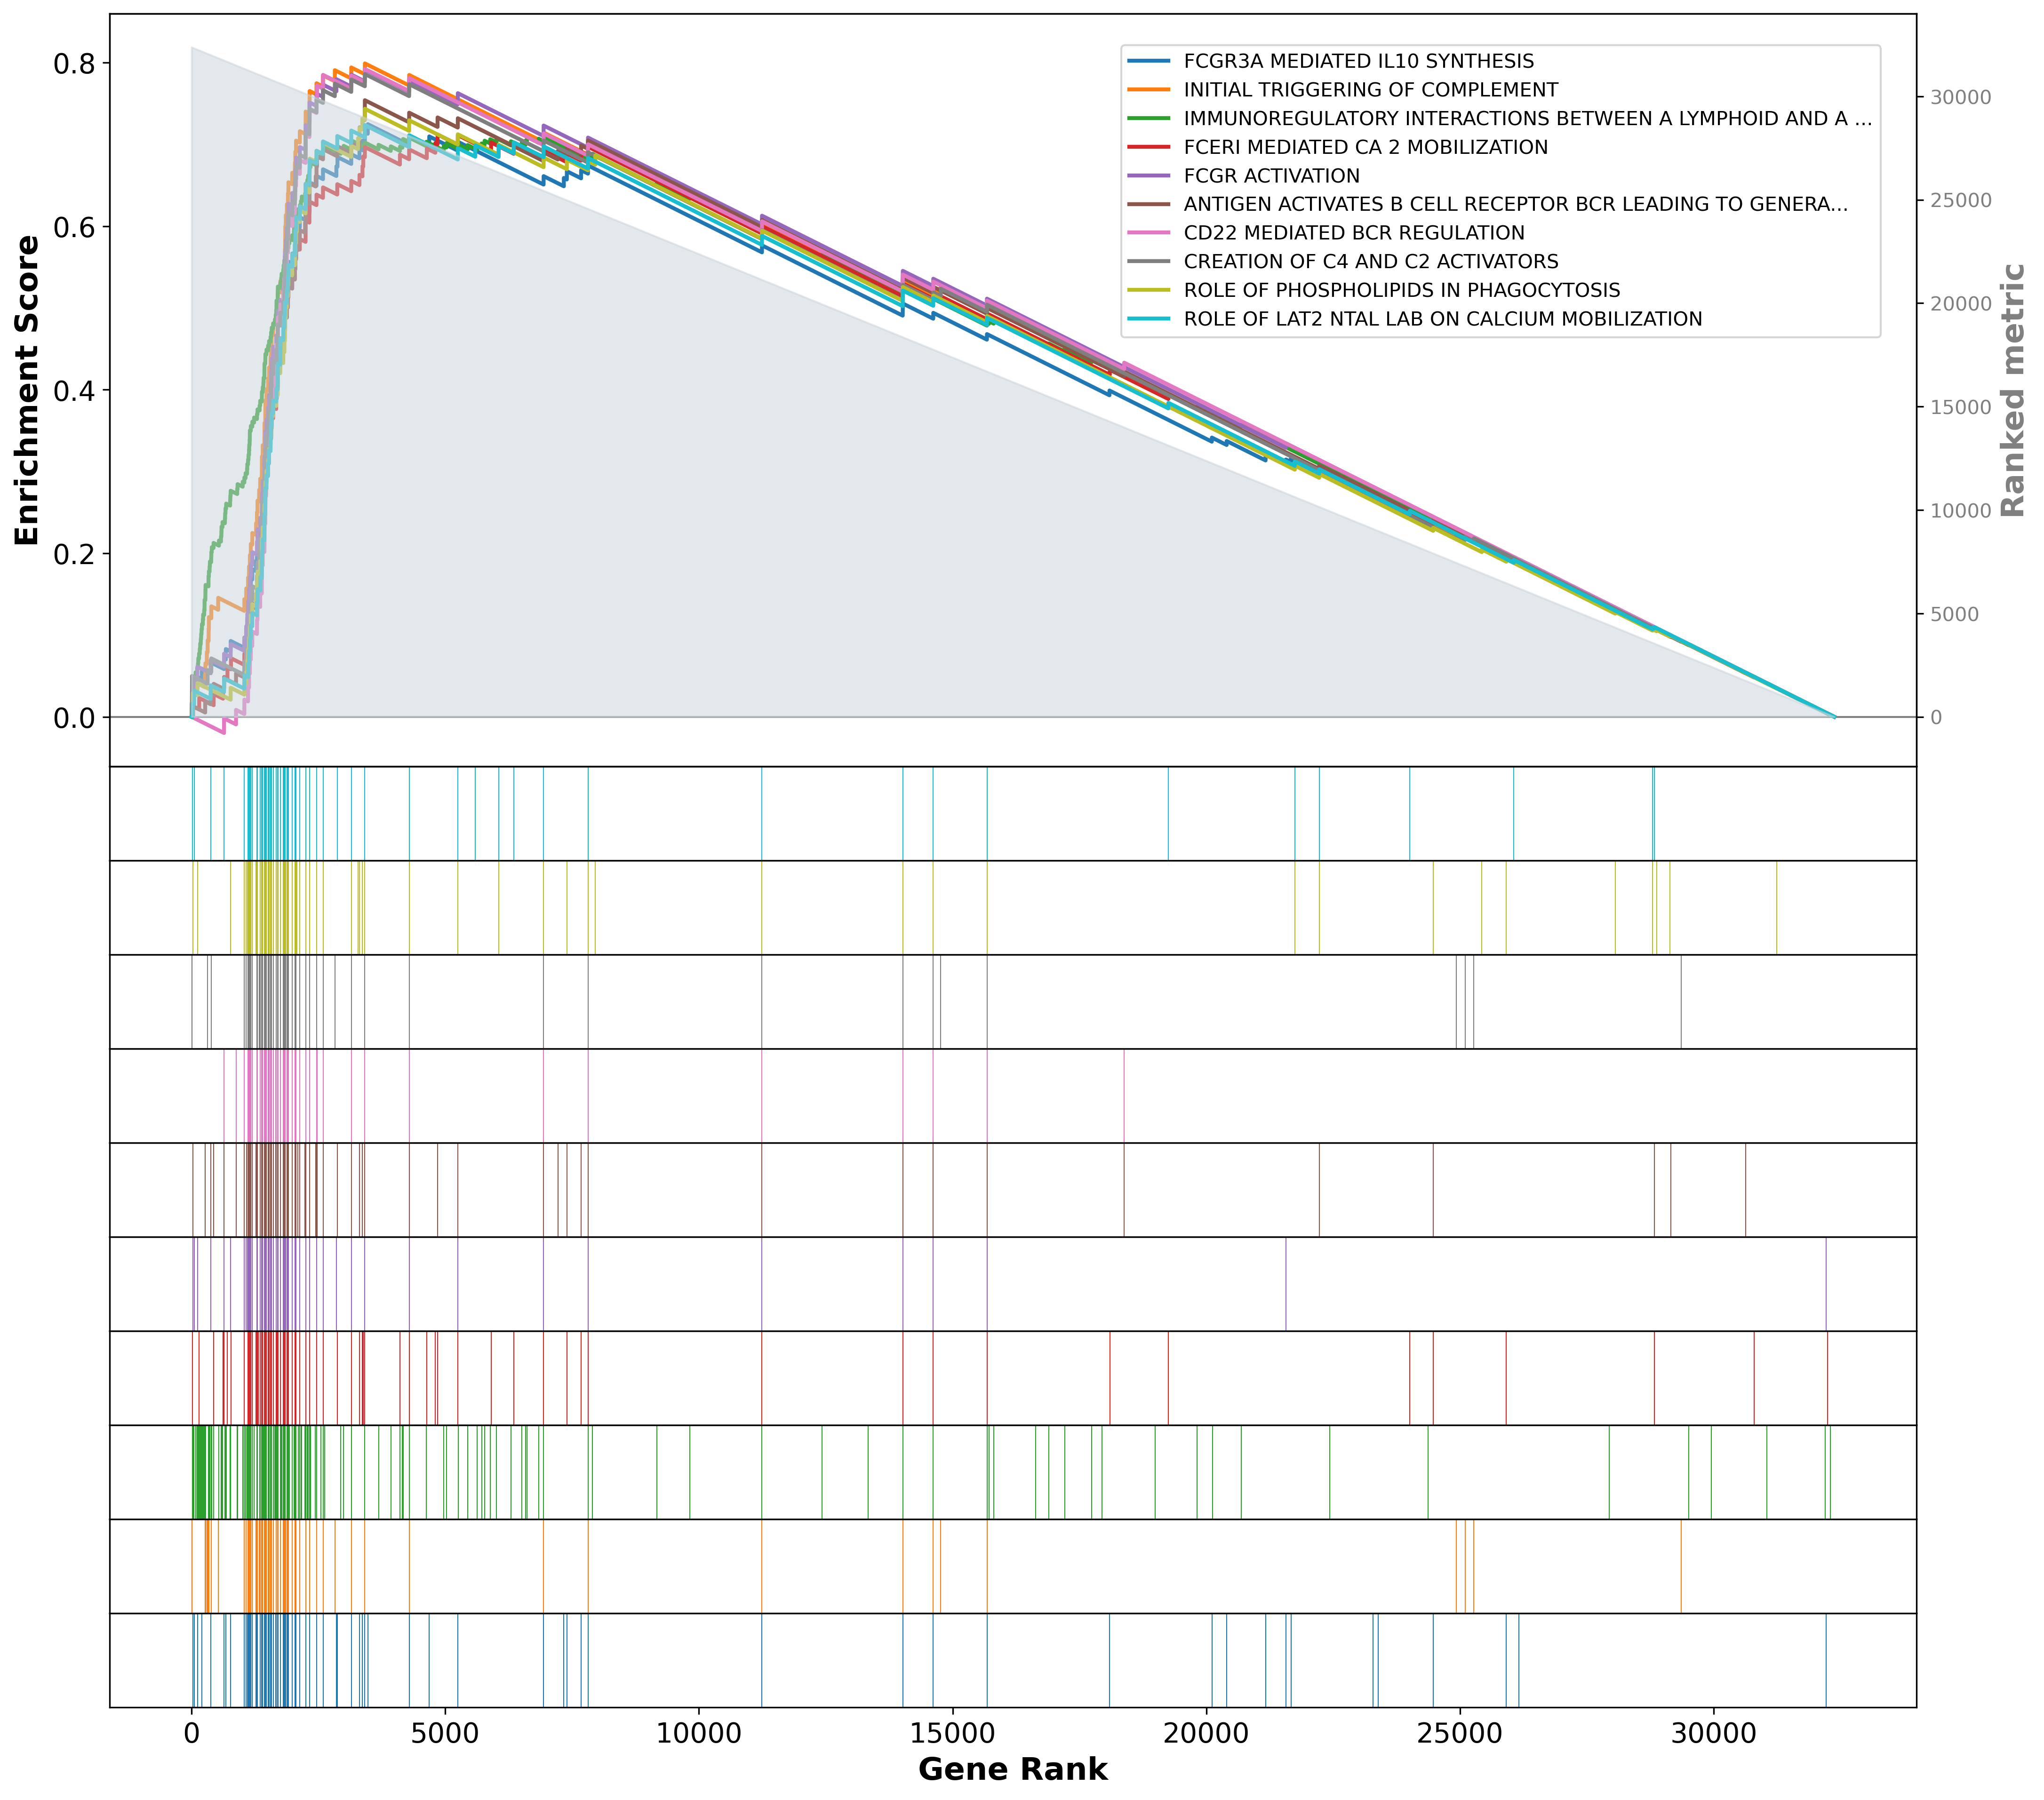
\includegraphics[width=\textwidth,keepaspectratio]{Sections/Network_I/Resources/selective_pruning/gsea/mesLike_10_top_manTerms.png}
    \caption[Mes 3: GSEA top 10 Reactome terms]{Top 10 GSEA terms with Reactome database for the Mes 3 group. Results interpretation in \cref{s:N_I:sel_tfs_mibc,s:ap:sel_prun_pi}.}
    \label{fig:ap:gsea_mesLike}
\end{figure}


\begin{figure}[!htb]
    \centering
    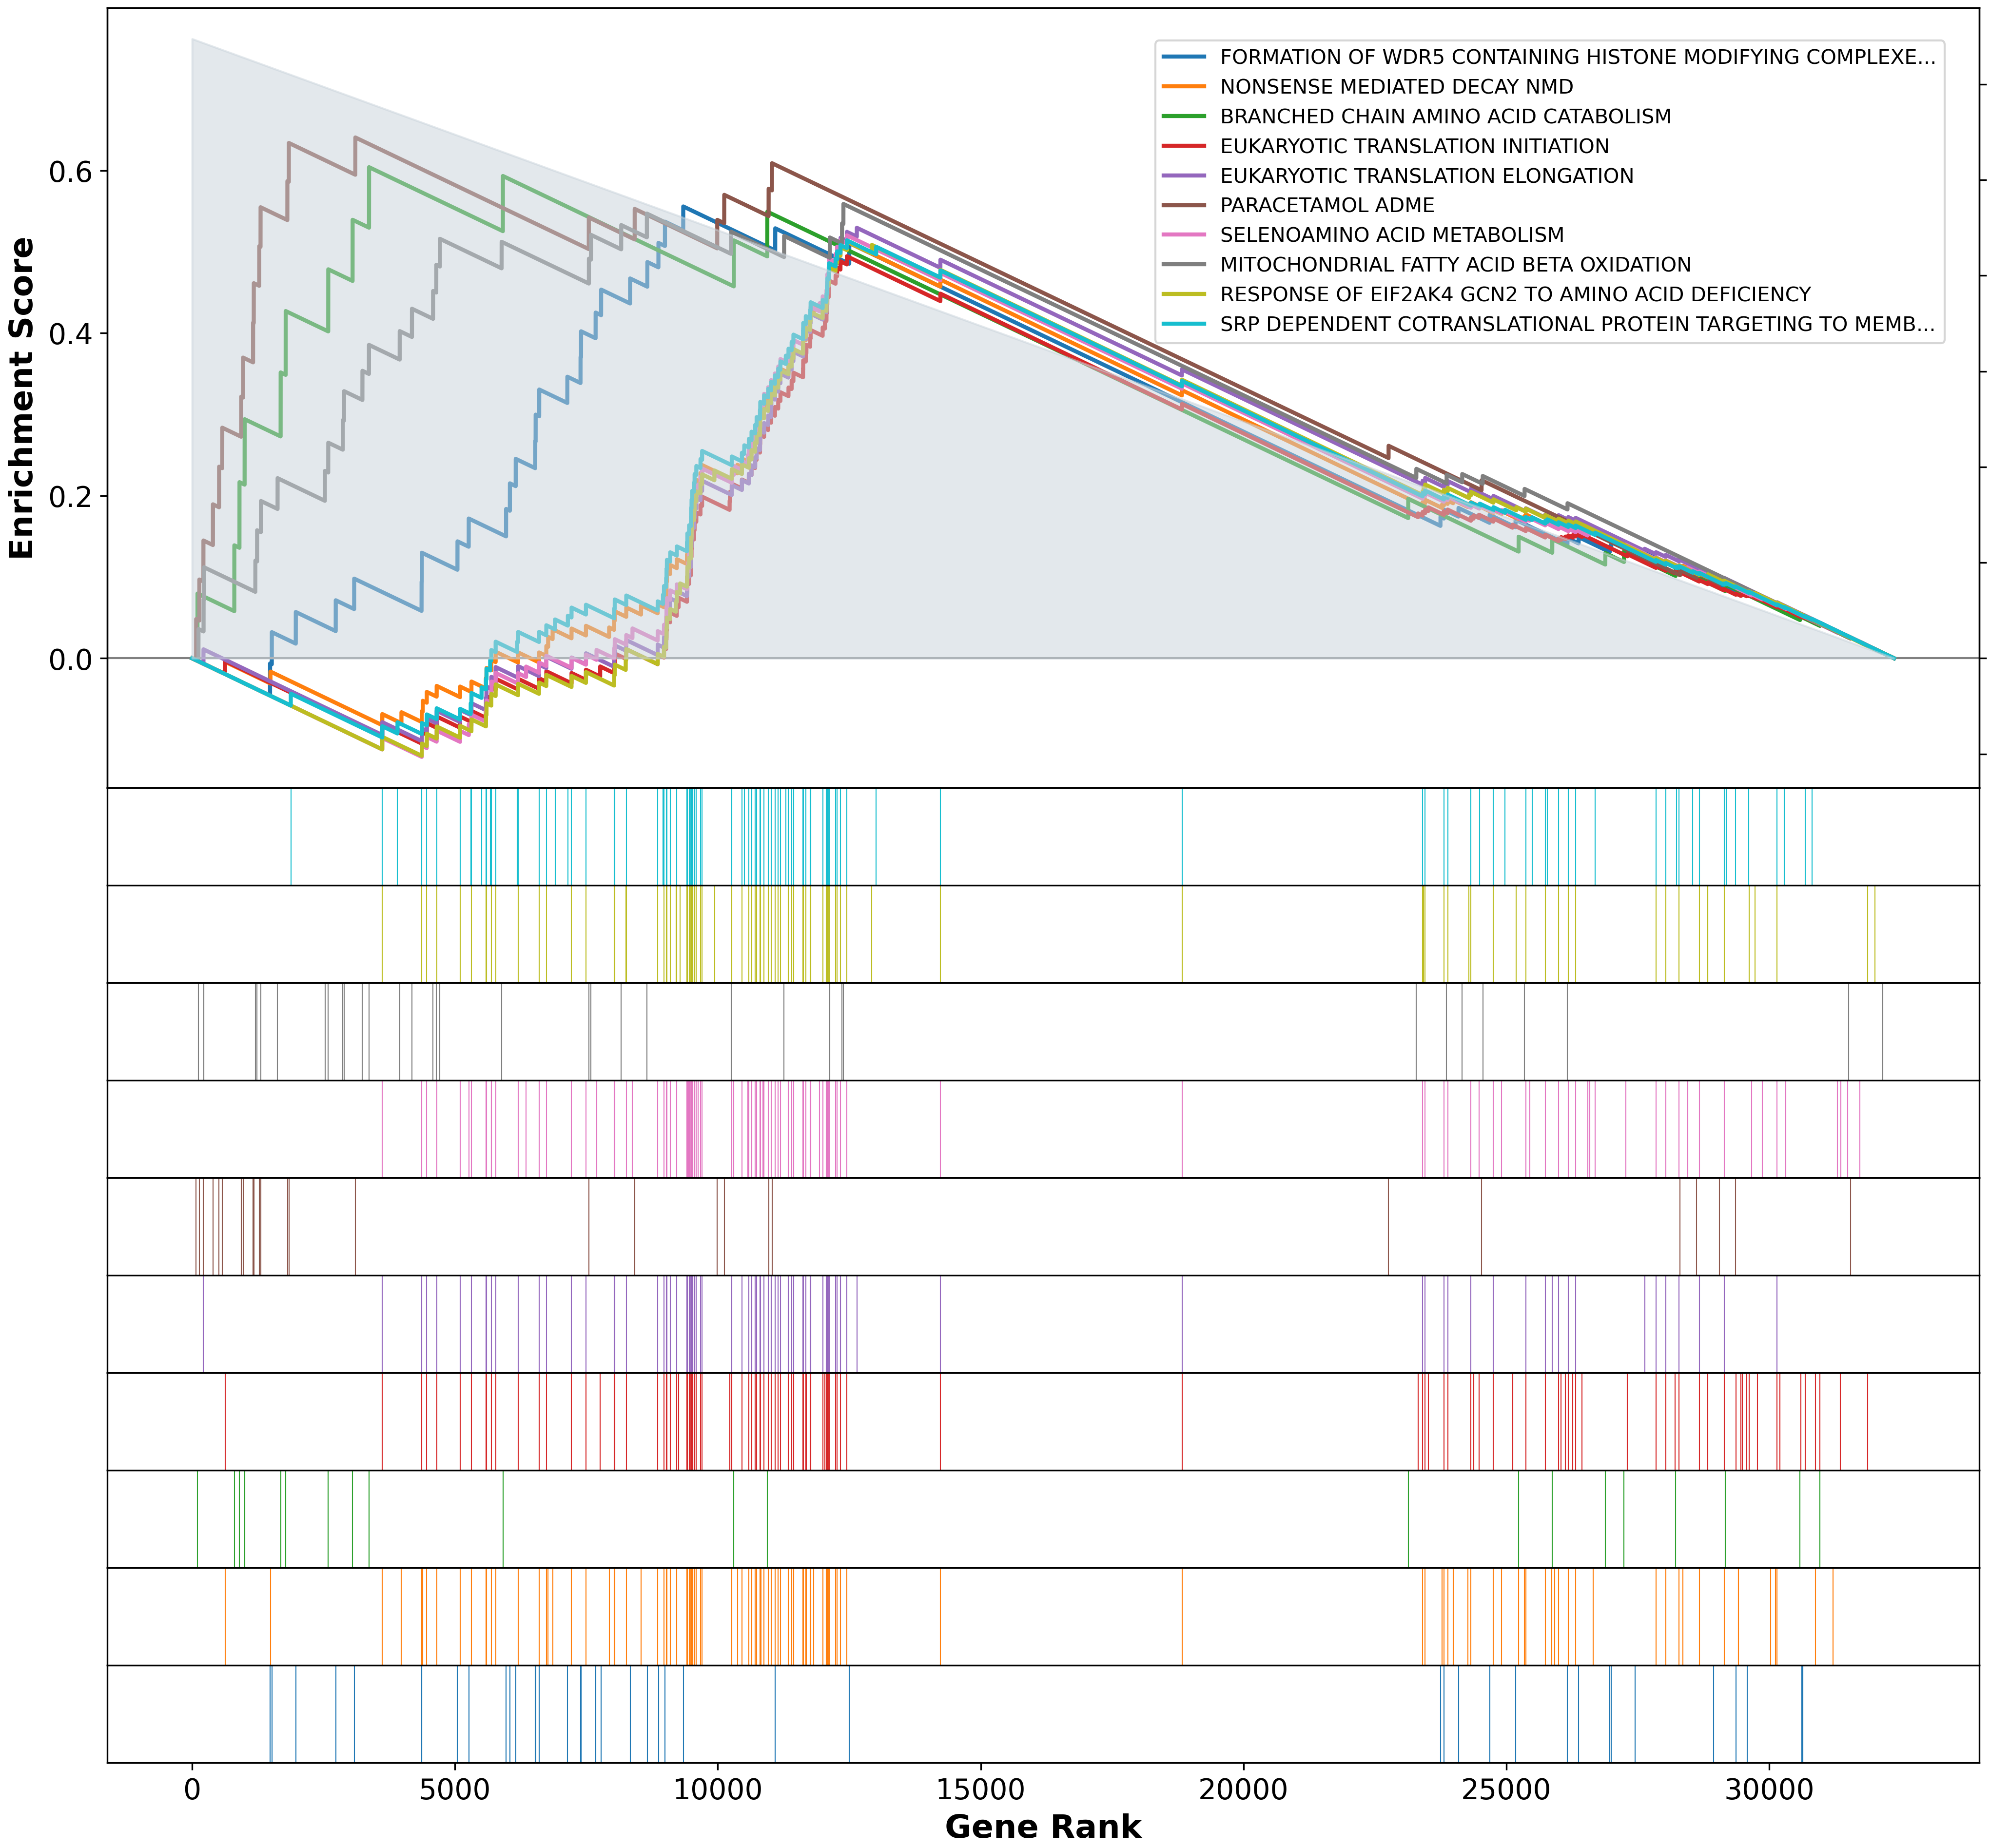
\includegraphics[width=\textwidth,keepaspectratio]{Sections/Network_I/Resources/selective_pruning/gsea/largeLuminal_10_top_manTerms.png}
    \caption[Lum 13: GSEA top 10 Reactome terms]{Top 10 GSEA terms with Reactome database for the Lum 13 group. Results interpretation in \cref{s:N_I:sel_tfs_mibc,s:ap:sel_prun_pi}.}
    \label{fig:ap:gsea_largeLuminal}
\end{figure}

\begin{figure}[!htb]
    \centering
    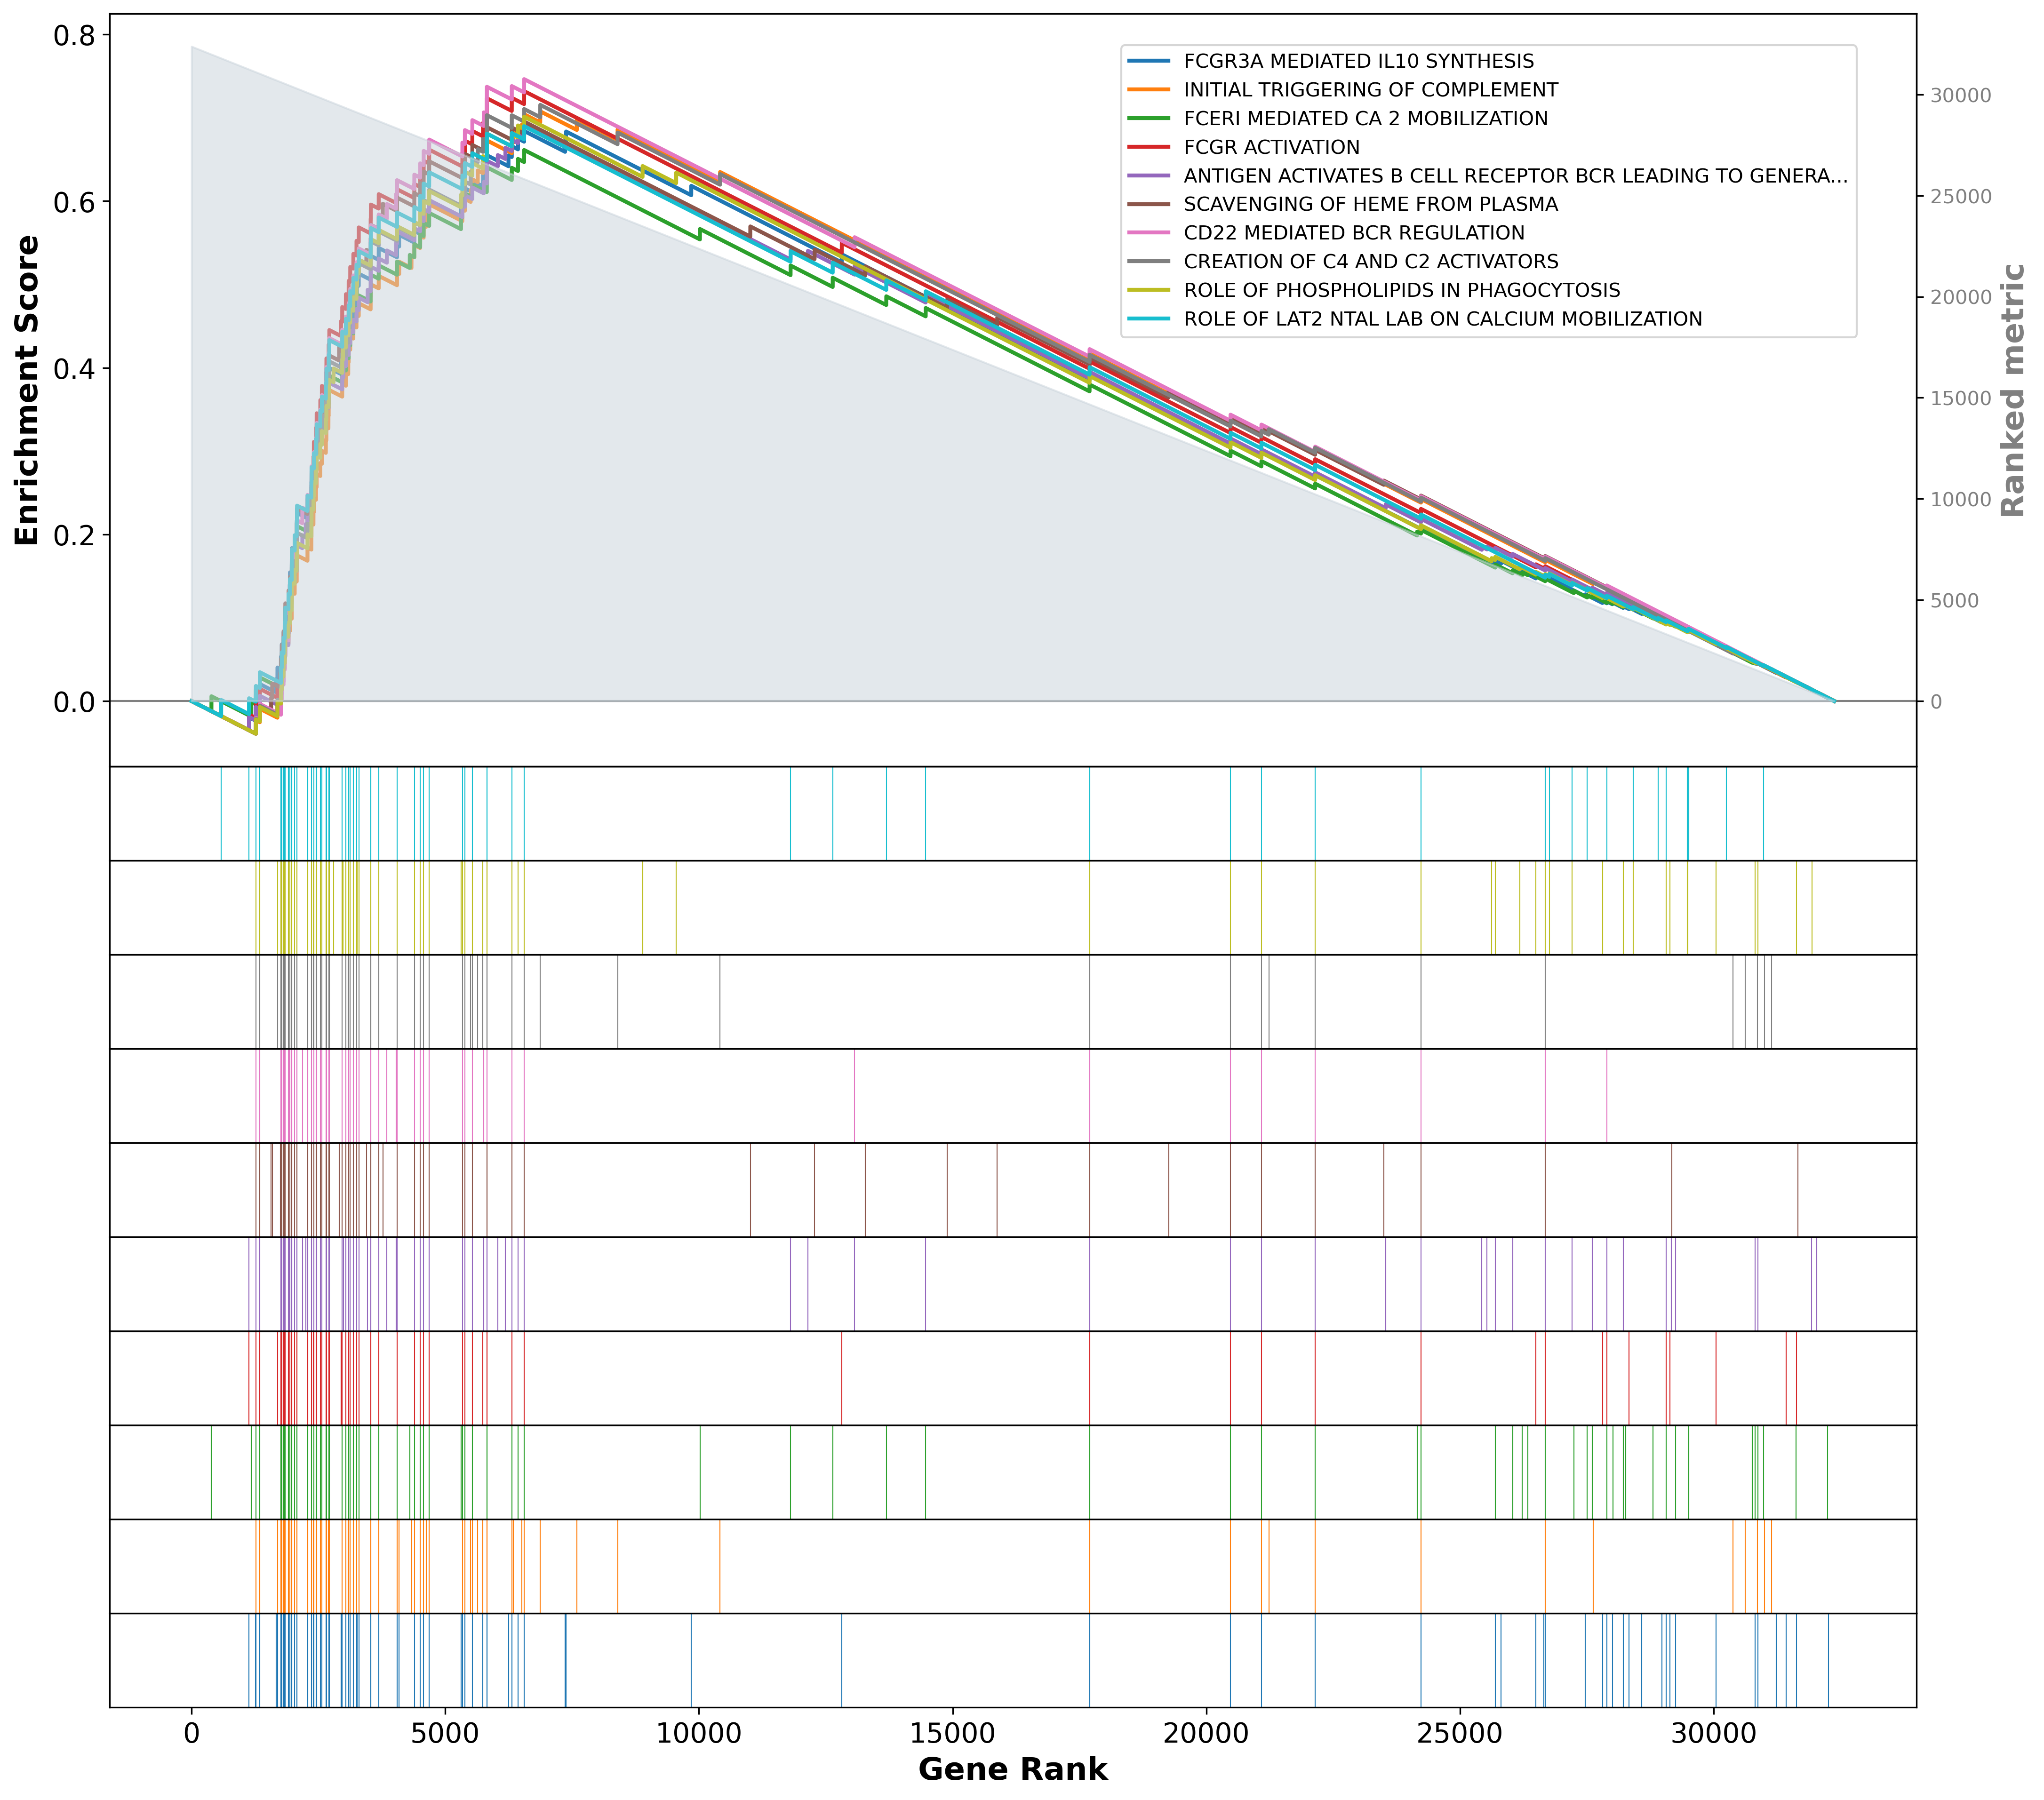
\includegraphics[width=\textwidth,keepaspectratio]{Sections/Network_I/Resources/selective_pruning/gsea/lumInf_10_top_manTerms.png}
    \caption[Lum 12: GSEA top 10 Reactome terms]{Top 10 GSEA terms with Reactome database for the Lum 12 group. Results interpretation in \cref{s:N_I:sel_tfs_mibc,s:ap:sel_prun_pi}.}
    \label{fig:ap:gsea_lumInf}
\end{figure}


% GSEA - hallmarks
\section{GSEA output (Hallmarks)} \label{s:ap:hallmarks}

This section supports the results presented in \cref{s:N_I:sel_tfs_mibc}, where the five subtypes were derived using the gene expression of the 98 TF identified through selective edge pruning, as discussed in \cref{s:N_I:sel_tfs}. The Pi plots used to rank the data can be seen in \cref{s:ap:sel_prun_pi}. In contrast to the main section, this GSEA analysis was performed using the Hallmark database.


\begin{table}[H]
  \centering
  \scriptsize
  \begin{tabularx}{\textwidth}{>{\hsize=1.5\hsize}X|>{\hsize=0.4\hsize}X|>{\hsize=0.4\hsize}X|>{\hsize=0.6\hsize}X|>{\hsize=0.4\hsize}X|>{\hsize=0.4\hsize}X}
    \toprule
    \textbf{Term} & \textbf{NES} & \textbf{FDR q-val} & \textbf{\# lead} & \textbf{\# matched} & \textbf{ratio} \\
    \midrule
    \multicolumn{6}{c}{\textbf{smallBasal}} \\
    \midrule
    MYC TARGETS V1 & 1.909 & 0 & 149 & 40 & 0.268 \\
    \midrule
    MITOTIC SPINDLE & 1.887 & 0 & 138 & 61 & 0.442 \\
    \midrule
    TGF BETA SIGNALING & 1.863 & 0 & 28 & 15 & 0.536 \\
    \midrule
    \multicolumn{6}{c}{\textbf{largeBasal}} \\
    \midrule
    KRAS SIGNALING UP & 2.384 & 0 & 132 & 104 & 0.788 \\
    \midrule
    \multicolumn{6}{c}{\textbf{lumInf}} \\
    \midrule
    CHOLESTEROL HOMEOSTASIS & 1.892 & 0 & 33 & 20 & 0.606 \\
    \midrule
    APOPTOSIS & 1.733 & 0 & 61 & 37 & 0.607 \\
    \midrule
    \multicolumn{6}{c}{\textbf{largeLuminal}} \\
    \midrule
    DNA REPAIR & 1.617 & 0.004 & 77 & 12 & 0.156 \\
    \midrule
    PEROXISOME & 1.608 & 0.003 & 57 & 22 & 0.386 \\
    \midrule
    FATTY ACID METABOLISM & 1.552 & 0.004 & 71 & 38 & 0.535 \\
    \midrule
    PROTEIN SECRETION & 1.549 & 0.003 & 42 & 11 & 0.262 \\
    \midrule
    BILE ACID METABOLISM & 1.46 & 0.008 & 59 & 19 & 0.322 \\
    \bottomrule
  \end{tabularx}
  \caption[98 TF: summary of hallmarks pathways]{Normalised Enrichment Score (NES), False Discovery Rate (FDR) q-val, and lead gene statistics for different subtypes. The lead genes from a pathway are selected by GSEAY based on when the NES reached its peak.}
  \label{ap:tab:gsea_hallmark}
\end{table}

% Other supporting material
\section{Other supporting materials}

\begin{sidewaysfigure}
    \centering
    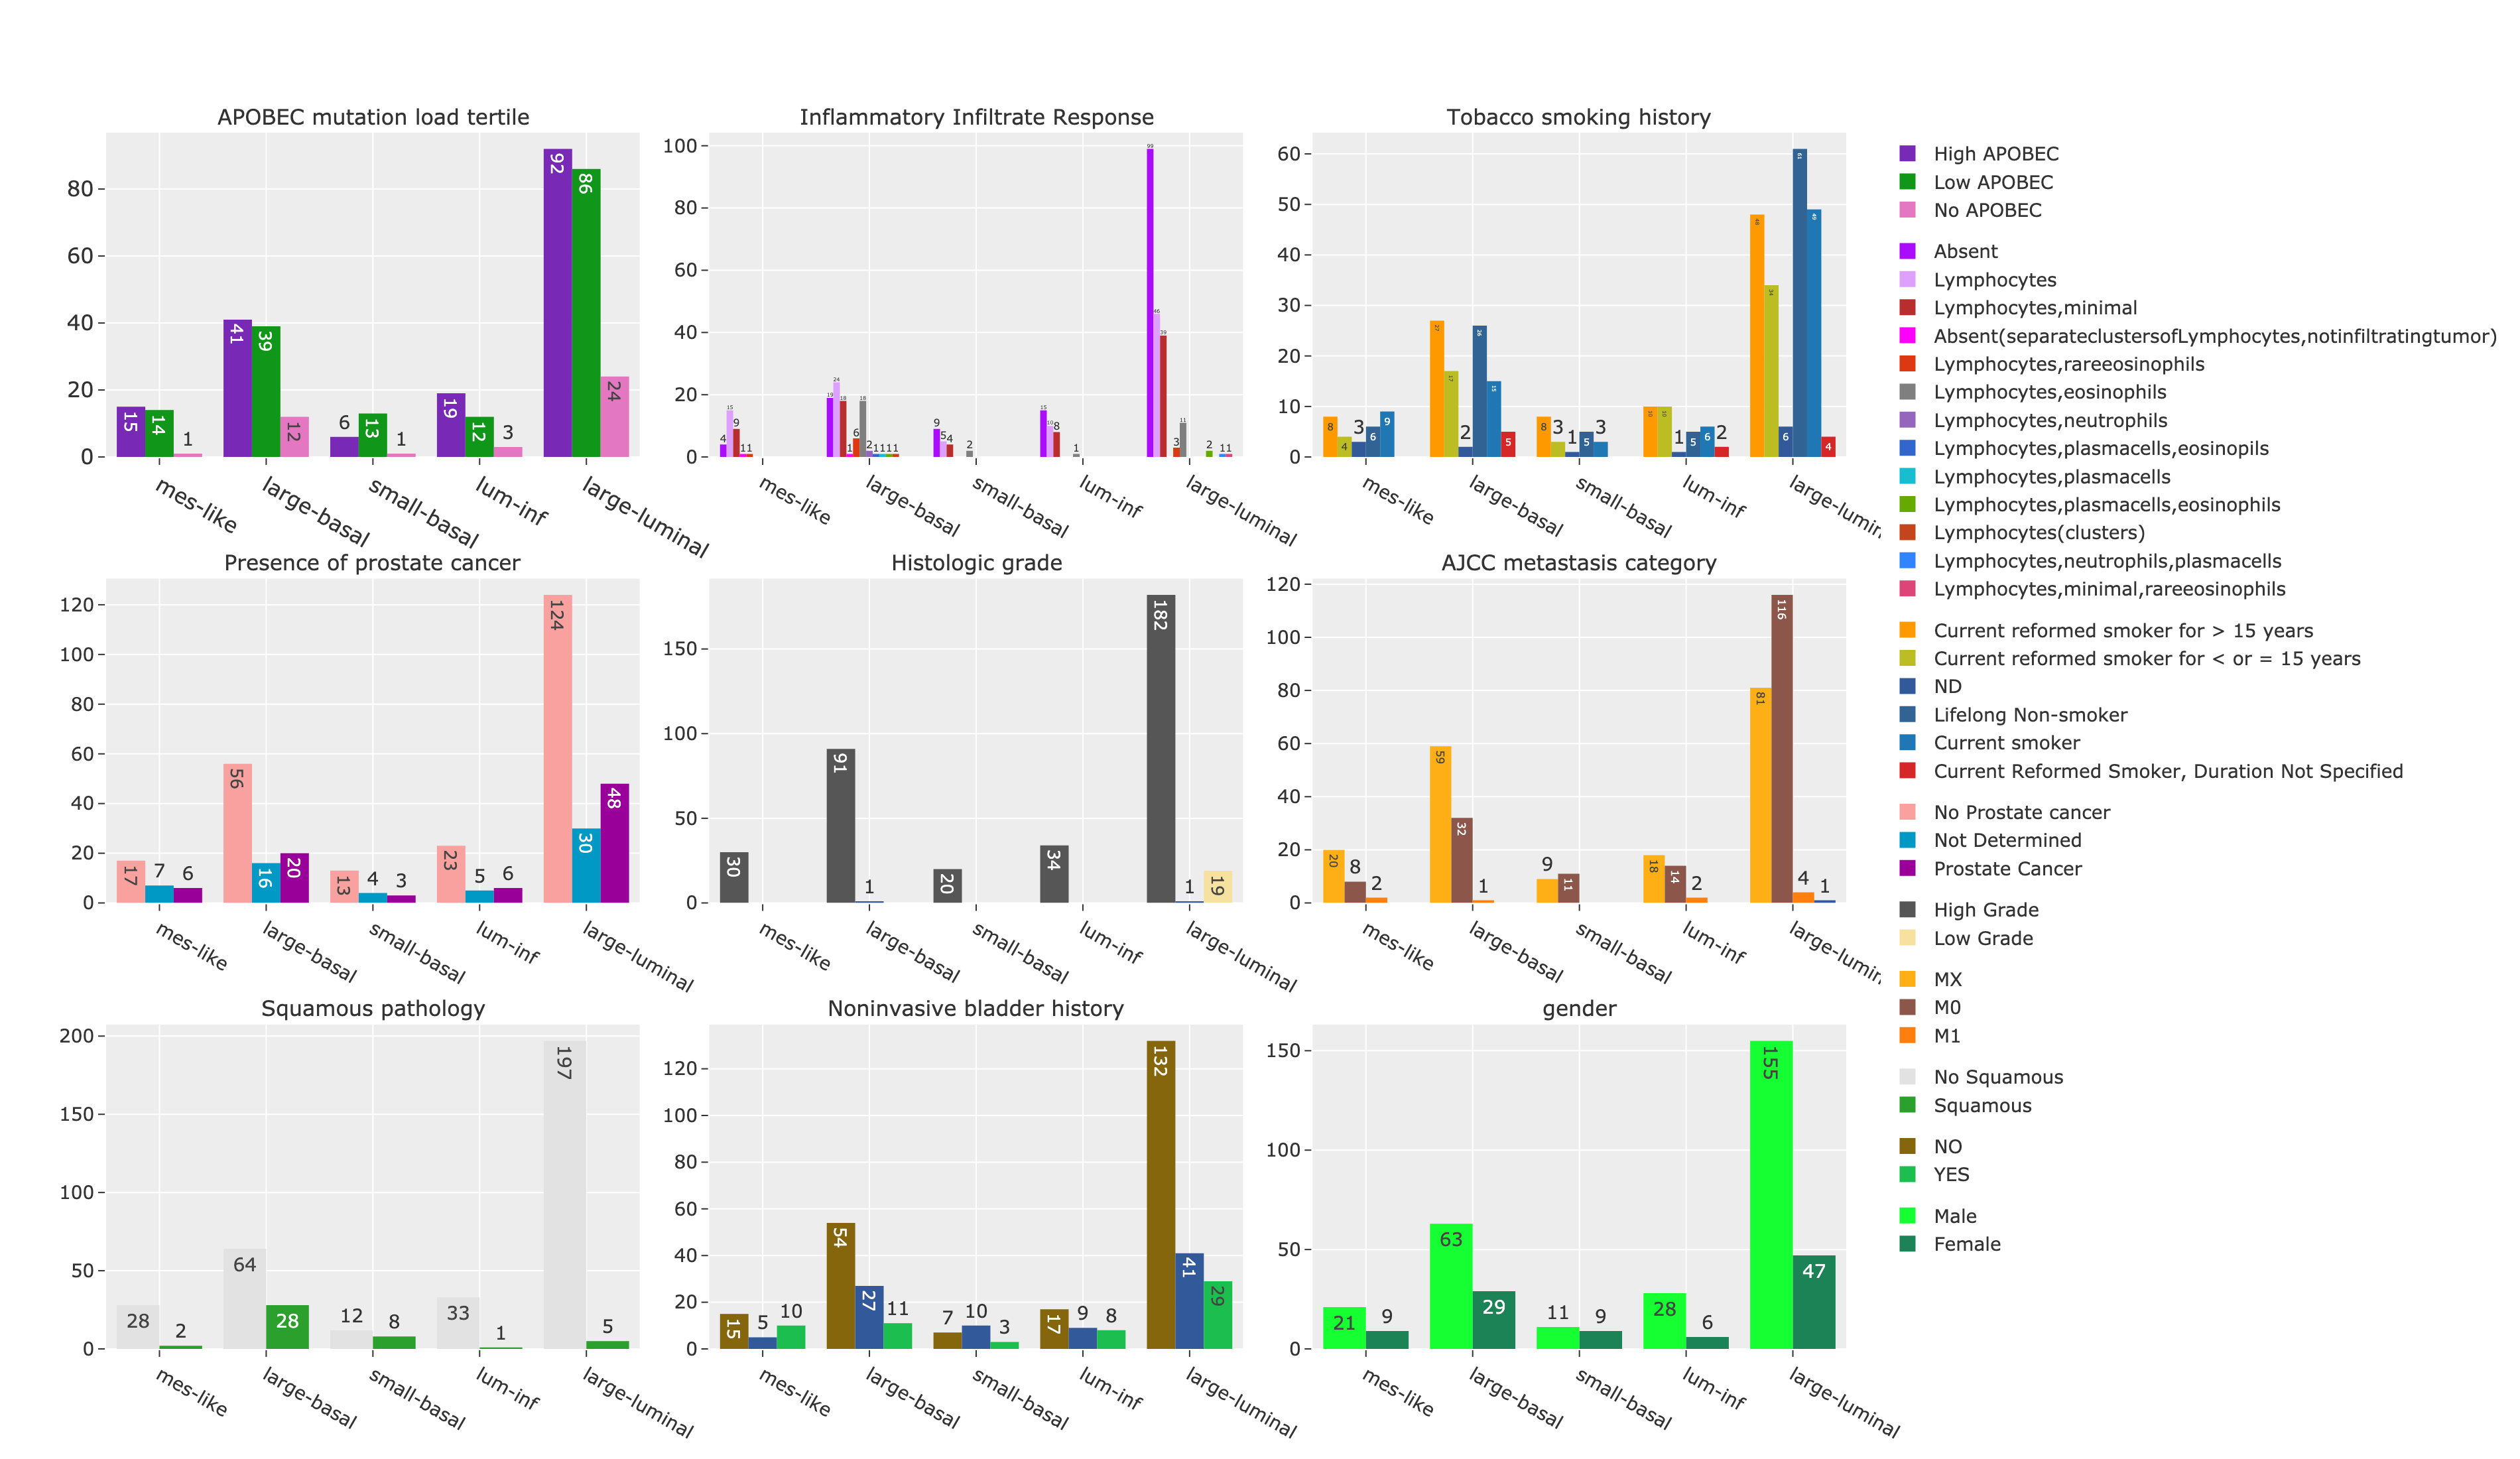
\includegraphics[width=1.0\textwidth,keepaspectratio]{Sections/Network_I/Resources/selective_pruning/sel_tfs/sel_tfs_tcga_meta.png}
      \caption[TCGA metadata and the groups derived from the 98 TF]{The metadata from TCGA \cite{Robertson2017-mg} across the subtypes derived from applying hierarchical clustering on the expression of the 98 TF from \cref{fig:N_I:sel_tfs}. The figure supports the analysis performed in \cref{s:N_I:sel_tfs_metadata}.}
    \label{fig:ap:sel_tfs_tcga_metadata}
\end{sidewaysfigure} 

\newpage 


\begin{sidewaysfigure}
    \centering
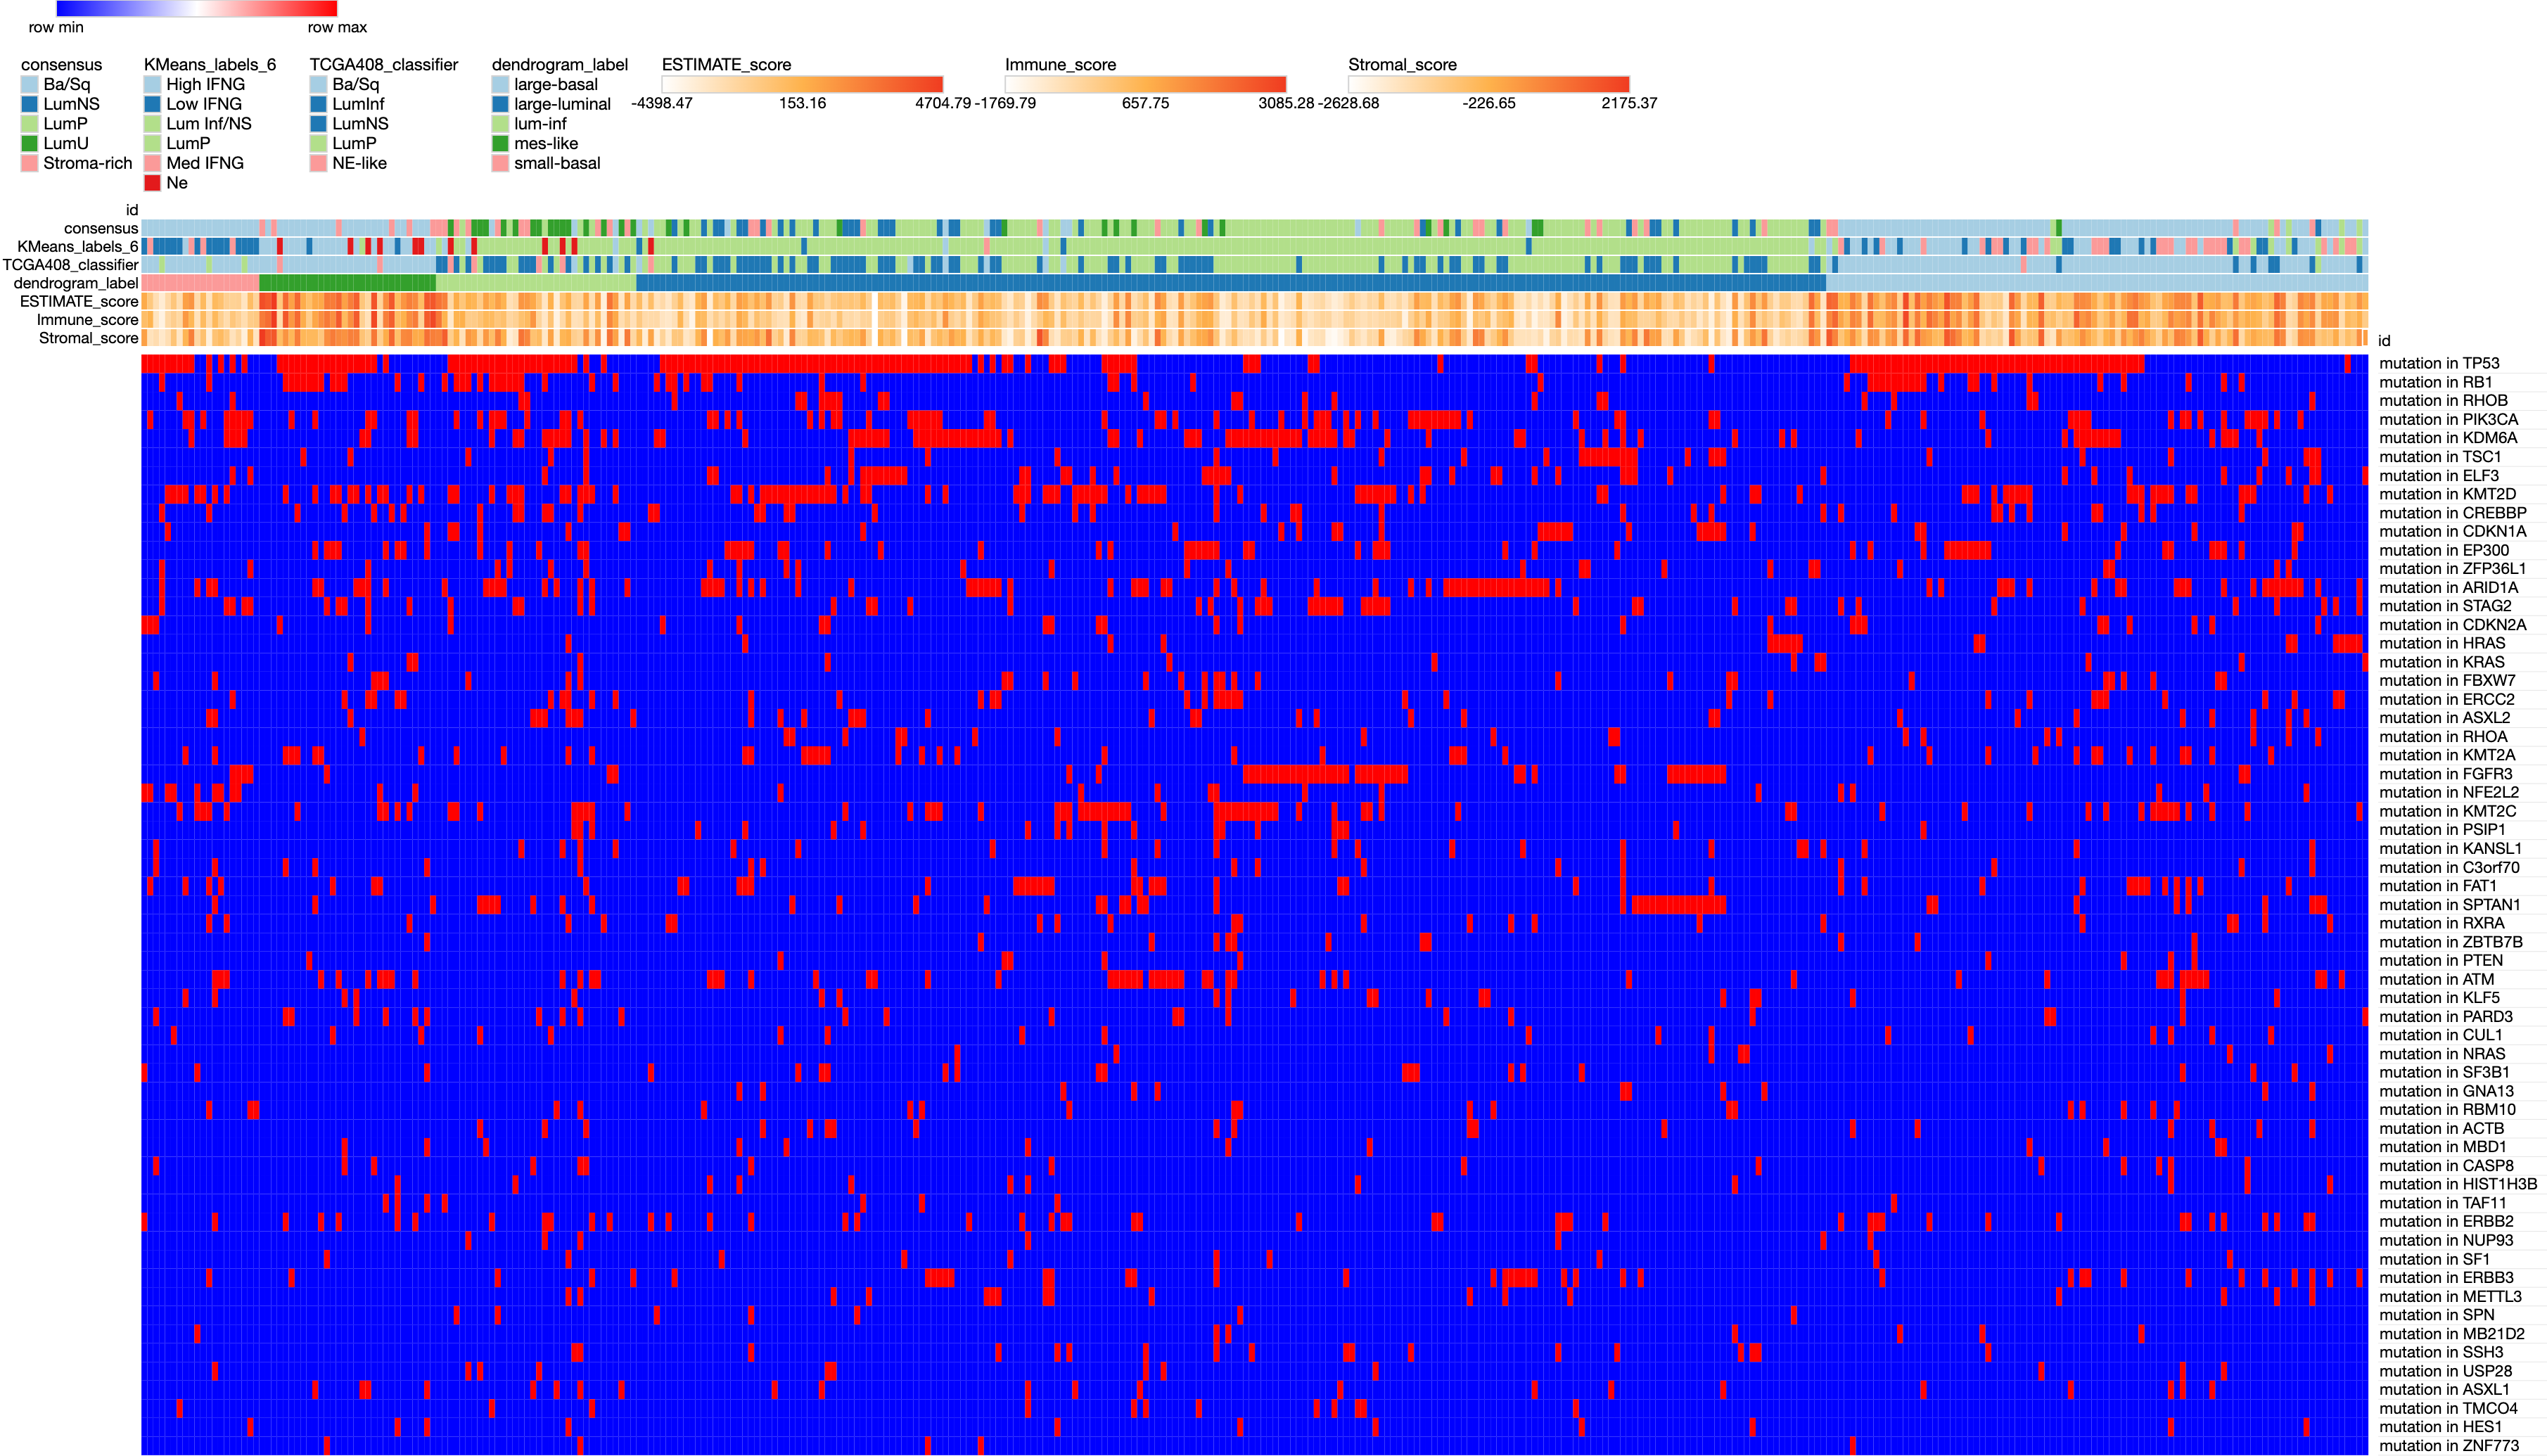
\includegraphics[width=1.0\textwidth,height=1.0\textheight,keepaspectratio]{Sections/Network_I/Resources/selective_pruning/sel_tfs/sel_tfs_mut_meta.png}
      \caption[98 TF: subgroups and somatic mutations]{Heatmap of binary somatic mutation across across the groups derived using the selective edge pruning. The figure show that there is no hint of relation between the subgroups and the mutations. The figure supports the analysis performed in \cref{s:N_I:sel_tfs_metadata}}
    \label{fig:ap:sel_tfs_tcga_meta_mut}
\end{sidewaysfigure}